 \input{include/twoside}
%\input{include/oneside}

\usepackage{include/tdk} % dafuq

\usepackage{ amssymb }

\input{include/notation}

\newcommand*{\bme}{Budapest University of Technology and Economics}
\newcommand*{\vik}{Faculty of Electrical Engineering and Informatics}

\newcommand*{\bmemit}{Department of Measurement and Information Systems}

\newcommand*{\vikdoctype}{MSc Thesis}
\newcommand*{\viktdklocation}{Budapest}
\newcommand*{\viktdkyear}{2017}

\newcommand*{\authors}{Authors}
\newcommand*{\advisors}{Supervisors}

\newcommand*{\authori}{László Márk Balogh}
\newcommand*{\authorihun}{Balogh László Márk}

\newcommand*{\advisori}{Vörös András}
\newcommand*{\advisorii}{dr. Bergmann Gábor}
\newcommand*{\advisoriii}{Farkas Rebeka}

\title{Complex Event Processing Based on Automata Theory}
\newcommand*{\titlepagetitle}{Complex Event Processing Based on Automata Theory}
\author{\authori}

\hypersetup{
  pdftitle={\thetitle},
  pdfauthor={\theauthor, \advisors: \advisori, \advisorii, \advisoriii}
}

%%% Local Variables:
%%% mode: latex
%%% TeX-master: "../main"
%%% End:



% Custom stuff, add it to the template later.
 \newcommand{\mytodo}[1]{}
 \renewcommand{\mytodo}[1]{{\color{red} TODO: {#1}}}

\usepackage{todonotes}


\usepackage{ cmll }

\lstdefinelanguage{Xtext}{
	morekeywords={grammar, with, hidden, generate, as, import, returns, current, terminal, enum},
	keywordstyle=[2]{\textbf},
	morecomment=[l]{//}, 
	morecomment=[s]{/*}{*/}, 
	morestring=[b]",
	tabsize=4}
\newcommand{\lstXtext}[1]{\lstinline[breaklines=true,language=Xtext,basicstyle=\listingsfontinline,mathescape,literate={\-}{}{0\discretionary{-}{}{}}]\S#1\S}


%Absolutely custom stuff for only myself
\newcommand{\redraw}{\mytodo{redraw this image with Power Point}}


% Comment in this line to remove todos
%\renewcommand{\todo}{}

%Tikz stuff 
\tikzstyle{rect} = [
	thick,
	inner sep=2mm,
	%minimum width=30mm,
	minimum height=10mm,
	align=center,
	draw=black,
	rectangle
]


%\usetikzlibrary{
%	arrows,arrows.meta,
%	shapes,shapes.geometric,shapes.misc,
%	chains, trees,
%	positioning,decorations.pathreplacing	
%}

\bibliography{references}

\begin{document}

\frontmatter

\thispagestyle{plain}

\includepdf[noautoscale]{thesis_topic}
\cleartorecto

\include{include/titlepage}

\tableofcontents

\begin{otherlanguage}{magyar}

  \paragraph*{Kivonat}
  \phantomsection
  \addcontentsline{toc}{chapter}{Kivonat}
  \thispagestyle{plain}

  A hagyományos kritikus rendszerekben gyakorta alkalmazott módszer a futási idejű ellenőrzés.
  Ennek célja olyan ellenőrző programok szintézise, melyek segítségével felderíthető egy kritikus komponens hibás, a követelményektől eltérő viselkedése a rendszer működése közben.
  Többek között ezt a célt szolgálja egy, a tanszéken fejlesztett keretrendszer is, amely élő modelleket használ és az azok fölött értelmezett modelltranszformációs szabályok segítségével definiálja a vizsgálandó temporális kifejezést.
  Modelltranszformációk helyességének ellenőrzése azonban algoritmikusan eldönthetetlen feladat általánosságban, így a definiált temporális viselkedéseket is nehéz formálisan vizsgálni.
  Az irodalomban többféle megközelítés létezik a temporális viselkedések definiálására és többféle formalizmust is definiáltak automata alapokon.
  Ezekben közös, hogy az automaták többnyire jól vizsgálhatóak algoritmikusan, az általuk definiált és elfogadott nyelvekkel kapcsolatban lehetőség van formális analízisre és ellenőrzésre.
  
  Ebben a dolgozatban megvizsgálom az irodalomban ismert legfontosabb automataelméleti megközelítéseket, és ez alapján kiterjesztem a tanszéki keretrendszert a paraméteres temporális viselkedések automata elméleti reprezentációjával.
  Bemutatom egy automata reprezentáció implementációját amely alkalmas paraméteres és temporális tulajdonságok ellenőrzéséhez. 
  Elemzem a megoldást kifejezőerő szempontjából, és megvizsgálok egy mérnöki leíró nyelvet és annak leképzését automata reprezentációra.
  Ezen felül bemutatom az alapvető koncepcionális megoldását egy paraméteres temporális automata végrehajtónak, és a néhány ehhez szükséges, általam kidolgozott adatszerkezetet.
  
  \paragraph{Kulcsszavak} véges állapotú automata, időzített automata, paraméteres időzített automata, Futásidejű verifikáció, komplexesemény-feldogozás, reguláris kifejezések
\end{otherlanguage}

\cleardoublepage

\paragraph*{Abstract}
\phantomsection
\addcontentsline{toc}{chapter}{Abstract}
\thispagestyle{plain}

In traditional safety-critical systems, runtime verification is a frequently used
method. The goal of runtime verification is to synthesize verification components, which
can detect the possible failures of the components. Over the last few years, researchers
of my department have started developing a framework called VIATRA-CEP being able
to support the runtime analysis and verification of complex systems. This framework
uses live models, and defines the temporal expressions by model transformation rules
over these live models. Verification of model transformations are generally algorithmically undecidable therefore it is hard to analyze these temporal behaviors. 
Various approaches exist in the literature supporting the definition of temporal behaviors, and many of them are defined based on automata theory.
Automata are usually easier to analyze algorithmically as the accepted languages of these automata can be formally analyzed.

In this thesis various automata based property representations are overviewed,
and a possible extension of the VIATRA-CEP framework is outlined. An automata
representation implementation for the analysis of parametric and temporal behavior is examined. The
solution is analyzed in terms of expressiveness, and a mapping from a high level domain
specific language to this automata representation is introduced.
An automaton executor implementation is also overviewed, alongside with the data structures which are required for the parametric timed execution. 


\paragraph{Keywords} finite state machine, timed automata, parametric timed automata, Runtime verification, complex event processing, regular expressions

%%% Local Variables:
%%% mode: latex
%%% TeX-master: "main"
%%% End:


\begin{otherlanguage}{magyar}

  \chapter*{Hallgatói nyilatkozat}
  \phantomsection
  \addcontentsline{toc}{chapter}{Hallgatói nyilatkozat}
  \thispagestyle{plain}

  Alulírott \textbf{\authorihun} szigorló hallgató kijelentem, hogy ezt
  a dolgozatot meg nem engedett segítség nélkül, saját magam
  készítettem, csak a megadott forrásokat (szakirodalom, eszközök stb.)
  használtam fel. Minden olyan részt, melyet szó szerint, vagy azonos
  értelemben, de átfogalmazva más forrásból átvettem, egyértelműen, a
  forrás megadásával megjelöltem.

  Hozzájárulok, hogy a jelen munkám alapadatait (szerző(k), cím, angol
  és magyar nyelvű tartalmi kivonat, készítés éve, konzulens(ek) neve) a
  \textls{BME} \textls{VIK} nyilvánosan hozzáférhető elektronikus
  formában, a munka teljes szövegét pedig az egyetem belső hálózatán
  keresztül (vagy hitelesített felhasználók számára)
  közzétegye. Kijelentem, hogy a benyújtott munka és annak elektronikus
  verziója megegyezik. Dékáni engedéllyel titkosított diplomatervek
  esetén a dolgozat szövege csak 3~év eltelte után válik hozzáférhetővé.

  \vspace{4ex}

  \noindent Kelt: \viktdklocation, \csname @date\endcsname

  \vspace{20ex}

  \hfill\begin{minipage}{0.4\linewidth}
    \centering\hbox to \linewidth{\cleaders\hbox{.}\hfil}\par
    \centering\authorihun\par
  \end{minipage}

\end{otherlanguage}

%%% Local Variables:
%%% mode: latex
%%% TeX-master: "main"
%%% End:

\mainmatter

\chapter{Introduction}
\label{chap:intro}

Assuring the correctness of critical systems is important as their failure might cause huge loss.
Nowadays the application of runtime verification is an emerging trend in the safety-critical and cyber-physical systems, to increase safety, as in case of a failure in these systems there is always a large amount of money or human lives at stake. 

However, designing and implementing runtime analysis is a complex task. The manual implementation is expensive, the resulting system will be complex, and the faultless operation is not assured.
There is a huge need for languages to define the requirements of safety-critical systems.
Moreover, there is also a need for certainty in the verification component, and this need makes design time verification and formal model checking desirable. 

The motivation of my work is to enhance the available approaches and take one step towards an expressive formalism to support runtime analysis of complex systems.
The goal of the paper is to find an intermediate language which can bridge the gap between system level requirements and their runtime verification.

Contributions in this paper: 
I briefly overview the architecture of the VIATRA-CEP framework.
I introduce multiple automata and regular expression formalisms, and specify transformations from the regular expressions to the automata. 
And lastly, I go through the implementation of these formalisms and transformations, and show the transformations from the language of VIATRA-CEP to one of the previously mentioned formalism.
\chapter{Background}
\label{chap:background}

System development is a complex process, therefore it needs to be supported by various tools and algorithms. In this chapter I will introduce the background of our work \citep{tdk2015} and my previous BSc thesis \citep{bsc_thesis} towards an approach supporting correct system design.

\section{Development methods}

Traditional software development methods often use informal specifications to support system, architecture and component level designs -- which may also be informal. This can easily result in higher verification costs or faulty systems, making them suboptimal choices for safety-critical software development. In order to introduce some level of formality and allow manageable, hierarchical software testing procedures, the V model was developed.

\begin{figure}
	\centering
	\begin{tikzpicture}[
	start chain=going below,
	squarednode/.style={
		rectangle,
		draw=black,
		very thick,
		minimum height=1.5cm,
		text width=2.5cm,
		inner sep=2mm,
		align=center	
	},
	every loop/.style={
		looseness=2,
		text width=2cm	
	}
	]
	\node[squarednode] (D1) {Requirements};
	\node[squarednode] (D2) [below = of D1, xshift = 1cm] {Architecture design};
	\node[squarednode] (D3) [below = of D2, xshift = 1cm] {Component design};
	\node[squarednode] (I)  [below = of D3, xshift = 2.5cm] {Implementation};
	\node[squarednode] (V3) [above = of I , xshift = 2.5cm] {System V\&V};
	\node[squarednode] (V2) [above = of V3, xshift = 1cm] {Architecture V\&V};
	\node[squarednode] (V1) [above = of V2, xshift = 1cm] {Unit V\&V};
	\draw[thick,->] (D1) -- (D2) node [midway, left, align=right] {Refine};
	\draw[thick,->] (D2) -- (D3) node [midway, left, align=right] {Refine};
	\draw[thick,->] (D3) -- ( I) node [midway, right, align=left] {};
	\draw[thick,<-] ( I) -- (V3) node [midway, right, align=left] {};
	\draw[thick,<-] (V3) -- (V2) node [midway, right, align=left] {Use};
	\draw[thick,<-] (V2) -- (V1) node [midway, right, align=left] {Use};
	\draw[thick,->] ($(D1.east)+(0,.4)$) -- ($(V1.west)+(0,.4)$) node [midway, above] {Transform};
	\draw[thick,->] ($(D2.east)+(0,.4)$) -- ($(V2.west)+(0,.4)$) node [midway, above] {Transform};
	\draw[thick,->] ($(D3.east)+(0,.4)$) -- ($(V3.west)+(0,.4)$) node [midway, above] {Transform};
	\draw[thick,<-] ($(D1.east)-(0,.4)$) -- ($(V1.west)-(0,.4)$) node [midway, above] {Test};
	\draw[thick,<-] ($(D2.east)-(0,.4)$) -- ($(V2.west)-(0,.4)$) node [midway, above] {Test};
	\draw[thick,<-] ($(D3.east)-(0,.4)$) -- ($(V3.west)-(0,.4)$) node [midway, above] {Test};
	\end{tikzpicture}
	\caption{The traditional V model\citep{vmodel}}
	\label{fig:intro:vmodel}
\end{figure}

\cref{fig:intro:vmodel} shows the stages of development, where a symbolic ``V'' shows the progress of the workflow. The project definition stages on the left side begin with the development of a concept of operations, continue with requirements and architecture, and detailed design. The implementation stage is shown across the base of the ``V''. The right side shows the testing and implementation stages of a system, with an upward-pointing arrow for progress of the workflow\citep{vmodel}. 

The V model is the basic scheme of software development. In the left of the figure, we proceed by decomposing the specification into an architecture level design, and the architectural design into component-level designs. Every level of decomposition has it's own specification. After the implementation process, each level of the implementation is verified with respect to the corresponding specification. This verification can be done incrementally, parallel  with the implementation process.

\subsection{Model driven software development}

Model-driven software development (MDSD) emphasizes problem solving by the development and maintenance of models describing the system being designed. MDSD heavily relies on automated code and documentation generation based on the models of components or the overall model of the system. 

Modeling has the advantage of introducing abstractions, thus reducing the complexity of the development process, by dividing it into smaller phases. Code generation guarantees that the code will inherit the properties that can be directly derived from the model, while reducing the costs by eliminating unnecessary round-trip engineering. The generation of documentation also results in the always up-to-date description of components, stored together with the requirements and the model. Furthermore, model-based approaches have the advantage of easier testability, or if the model is formal enough then formal verification might be applicable. This is especially important for the development of safety-critical systems, making MDSD notably widespread in such areas.

Various methods and tools are available for the generation of test cases and monitoring components from models, as well as for formally verifying certain properties. These tools usually support the modeling formalisms used in their application domain.

MDSD will usually result in a software life cycle model for component-based systems\citep{ymodel}, which is based on the V model.

\subsection{Y model} 

\begin{figure}
	\centering
	\begin{tikzpicture}[
	start chain=going below,
	squarednode/.style={
		rectangle,
		draw=black,
		very thick,
		minimum height=1.5cm,
		text width=2.5cm,
		inner sep=2mm,
		align=center
	},
	every loop/.style={
		looseness=2,
		text width=2cm
	}
	]
	\node[squarednode] (D1) {System\\Design Model};
	\node[squarednode] (D2) [below = of D1, xshift = .2cm] {Architecture\\Design Model};
	\node[squarednode] (D3) [below = of D2, xshift = .2cm] {Component\\Design Model};
	\node[squarednode] (V1) [right = 3cm of D1] {System\\V\&V Model};
	\node[squarednode] (V2) [below = of V1, xshift = -.2cm]{Architecture\\V\&V Model};
	\node[squarednode] (V3) [below = of V2, xshift = -.2cm] {Component\\V\&V Model};
	\node[squarednode] (GC) at ($(D3)!0.5!(V3)$) [yshift=-3.5cm, text width=5.5cm] {Design + V\&V Artifacts\\(Source code, Glue code,\\Config. Tables, Test Cases,\\Monitors, Fault Trees, etc.)};
	\draw[thick,->] (D3.south) -- (GC.north -| D3) node [midway, left, align=right] {Code generation};
	\draw[thick,->] (V3.south) -- (GC.north -| V3) node [midway, right, align=left] {Test generation};
	\draw[thick,->] (D1) edge [loop left, align=right] node {Design rules} ();
	\draw[thick,->] (D2) edge [loop left, align=right] node {Design rules} ();
	\draw[thick,->] (D3) edge [loop left, align=right] node {Design rules} ();
	\draw[thick,->] (V1) edge [loop right, align=left] node {Formal methods} ();
	\draw[thick,->] (V2) edge [loop right, align=left] node {Formal methods} ();
	\draw[thick,->] (V3) edge [loop right, align=left] node {Formal methods} ();
	\draw[thick,->] (D1.south) -- (D2.north) node [midway, left, align=right] {Derive};
	\draw[thick,->] (D2.south) -- (D3.north) node [midway, left, align=right] {Derive};
	\draw[thick,<-] (V1.south) -- (V2.north) node [midway, right, align=left] {Use};
	\draw[thick,<-] (V2.south) -- (V3.north) node [midway, right, align=left] {Use};
	\draw[thick,<->] ($(D1.east)+(0,.4)$) -- ($(V1.west)+(0,.4)$) node [midway, above] {Transform};
	\draw[thick,<->] ($(D2.east)+(0,.4)$) -- ($(V2.west)+(0,.4)$) node [midway, above] {Transform};
	\draw[thick,<->] ($(D3.east)+(0,.4)$) -- ($(V3.west)+(0,.4)$) node [midway, above] {Transform};
	\draw[thick,<->] ($(D1.east)-(0,.4)$) -- ($(V1.west)-(0,.4)$) node [midway, above] {Test};
	\draw[thick,<->] ($(D2.east)-(0,.4)$) -- ($(V2.west)-(0,.4)$) node [midway, above] {Test};
	\draw[thick,<->] ($(D3.east)-(0,.4)$) -- ($(V3.west)-(0,.4)$) node [midway, above] {Test};
	\end{tikzpicture}
	\caption{An overview of the Y model}
	\label{fig:intro:ymodel}
\end{figure}

The Y model\citep{ymodel} is an extension of the V model\citep{randomwikipedialink3}, by automating code and test case generation. Much like the V model, the development process is partitioned vertically. Each level has its own modeling languages and models that are transformed to a verification model, on which verification methods such as testing can be applied. The results of the verification process can be traced back to the original models making iterative improvement possible. The top level is for high level system models, while the second level contains architectural models, and the third one is for component-based models. The component model provides input for the source code and configuration generation for the individual components. Test cases are paired with the source code and can be generated from the component verification models.


\subsection{Modeling languages on different levels of abstraction}

Model Driven Software Development methods require modeling languages to describe the behavior of systems and components. Engineering practices resulted a wide range of such languages over the years to support efficient product development. This allows the use of domain-specific languages, which leads to a shorter modeling process. The result is the need for complex model transformations before the verification can begin,
but since the domain-specific languages are tailored exactly to the problem, their usage is more efficient -- but requires expertise in the domain.  

Standardized modeling languages were developed like the UML (Unified Modeling Language\citep{uml}) and SysML (Systems Modeling Language\citep{sysml1}\citep{sysml2}).

\subsubsection{Class diagram}

In software engineering, a class diagram in the Unified Modeling Language (UML) is a type of static structure diagram that describes the structure of a system by depicting the system's classes, their attributes, operations (or methods), and the relationships among objects. It is also often applied at the system level design, as multiple components and their connection can be visualized with Class diagrams.

\subsubsection{Message Sequence Chart}

The formalism of Message Sequence Charts (MSC) describes the communication between components -- the order in which messages can occur\citep{msc}\citep{msc2}\citep{Klose2003}. The message interchange is usually represented by a graphical model. These charts can be used for high-level specification, design, trace-based testing or documentation. A collection of possible sequence charts can also describe a complete communication protocol between components. UML sequence diagrams were inspired by MSCs, but their semantics differs regarding some of the basic elements of the language such as lifelines and arrows\citep{mscuml}.

\subsubsection{Sequence diagram}

A Sequence Diagram is an interaction diagram that shows how processes operate with one another and in what order. It is a construct of a Message Sequence Chart. A Sequence Diagram shows object interactions arranged in time sequence. It depicts the objects and classes involved in the scenario and the sequence of messages exchanged between the objects needed to carry out the functionality of the scenario. Sequence diagrams are typically associated with use case realizations in the logical view of the system under development. Sequence diagrams are sometimes called event diagrams or event scenarios. Sequence diagrams can be used for system-level modeling, as it can represent the communication between the components. 


\subsubsection{Statechart}

Statecharts, also known as state machines are an extension of finite automata. There are various available syntaxes for statecharts (e.g. the one defined by UML\citep{stcuml}). The higher level concepts that were introduced include variables, actions, and hierarchically nested states. Event-driven execution is also possible by using signals as the triggers of transitions. Available variable types heavily depend on the concrete semantics of the chosen statechart language. Actions can usually be variable assignments, signal raises or the setting of timers. Hierarchy lets users organize system descriptions using a top-down approach. Support for hierarchy is introduced via nested states and parallel regions. States can also have entry and exit actions, which allows the description of common functionality in parent states\citep{stcmove}.%\\

Statecharts are usually developed in tools that support the graphical design of the model (e.g.: Yakindu\citep{yakinduu}, an Eclipse-based editor).
Statecharts are commonly used as a form of component description, as it can represent the behavior of components depending on its state.

\subsubsection{Activity Diagram}

Activity diagrams are graphical representations of workflows of stepwise activities and actions with support for choice, iteration and concurrency. In the Unified Modeling Language, activity diagrams are intended to model both computational and organizational processes (i.e. workflows). Activity diagrams show the overall flow of control, and therefore can be used at the system level description.

\section{Verification techniques} 

As modern society is becoming more and more dependent on safety-critical systems, the need for faultlessly working hardware and software increases. The development of safety-critical systems require extensive testing efforts. Validation and verification methodologies have been present in the development processes of such systems for a long time\citep{ieee1012}, but faster and more reliable approaches are needed. Validation assures that the requirements specified for the software meet the needs of the user -- as such, validation usually can be aided, but can’t entirely be done by software. The goal of verification is to analyze whether the specified requirements are met by the system. Methods for verification can be divided into two groups: design time verification and runtime verification. These approaches aren't exclusive, and their mutual use can support a more robust verification process.

\subsection{Design time verification}

Design time verification is a method used for finding errors of the system before deployment. Traditional software development methodologies usually rely on design time approaches. Verification methods can be applied on multiple levels, from small parts to the whole system. These processes check the compliance of the system against the specification of the appropriate level.%\\ \todo{This line break is strange}

Formal verification can also be used to give proof that the verified parts match the behavior described by the (also formal) specification. On the other hand, applying formal methods usually have higher costs, and the verification of complex systems can be impossible due to the phenomenon of state space explosion. As a result, a possible application of formal methods is to verify the correct behavior of system components, and not the entire system.

\subsection{Runtime verification}

Runtime verification is a method for the inspection of running systems. The motivation of the approach
is to reduce to complexity of the design time verification. 
As systems are getting larger, the application of formal methods are more and more limited as the resources needed for verification cannot be realized. This means that formal verification methods must verify an abstract model, not the deployed system itself. In addition, specifications are rarely complete, and design time methods can rarely handle hardware errors. %\todo{This line break is strange}

Runtime verification uses monitors to observe certain (usually critical) components, checking whether their operation violates properties described in the specification. The usage of monitoring components can result in significantly smaller monitors than the component itself as multiple levels of abstraction can be used, as long as the error states remain distinguishable. This has the advantage of detecting the erroneous operation of the system and allows systematic safety engineering to handle faults, or trigger an emergency shutdown if necessary.

The main advantages of runtime verification are the following:

\begin{itemize}
	\item Smaller computational complexity.
	\item Verification of the running implementation.
	\item Detection of previously not defined errors.
\end{itemize}

\section{Complex event processing}

\begin{figure}[h]
	\centering
	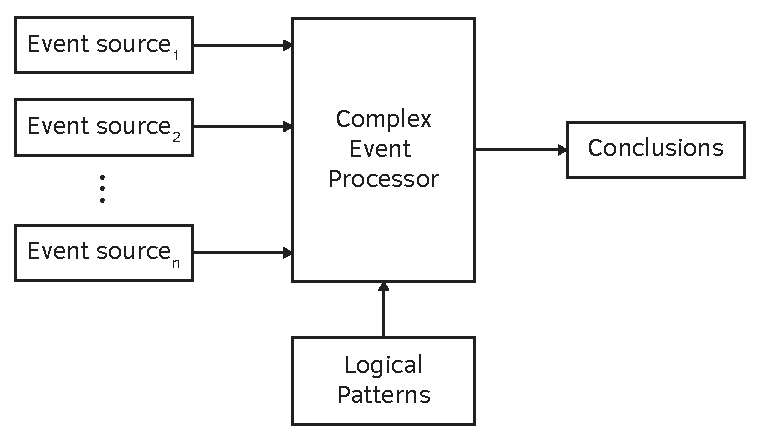
\includegraphics[width=0.6\linewidth]{figures/chapter_2/CEP}
	\caption{Complex event processing overview}
	\label{fig:intro:cep}
\end{figure}

Complex event processing (or CEP for short) is a method of tracking and analyzing streams of information and deriving conclusions. In a complex event processing environment, there can be multiple event sources, and with logical patterns given by a formalism, patterns (pattern matches) can be found in the incoming stream, e.g.~events followed by another events in some predefined sequence.

\subsection{Complex Event Processing Frameworks}
There are many Complex Event Processing Frameworks in the industry.

One of these tools is Drools\citep{drools} which is the leading Java based open-source rule engine. It is a hybrid chaining engine meaning that it can react to changes in data and also provides advanced query capabilities. Drools provides built-in temporal reasoning for complex event processing and is fully integrated with the jBPM project for BPMN2 based workflows.

Another well-known tool in the industry is Esper\citep{esper} which is an Event Stream Processing (ESP) and event correlation engine.
Targeted to real-time Event Driven Architectures (EDA), Esper is capable of triggering custom actions written as Plain Old Java Objects (POJO) when event conditions occur among event streams. It is designed for high-volume event correlation where millions of events coming in seconds. This amount of input would make it impossible to store all event in a classical database architecture and query them later.

\section{Runtime verification with CEP}
In this section the application of CEP for runtime verification is overviewed.
In general, system level runtime verification can be provided with the help of complex event processing. A complex event processing framework can monitor either the messaging between components and also the current state of the system and detect errors based on the specification of valid message sequences and valid states. 
The approach uses pattern matching to detect faulty operation of the system. Should illegal sequences occur, error handling operations (e.g.~restart or shutdown of a component or the whole system) can be applied to avoid the violation of safety criteria.

\subsection{Finite automaton }

\todo{How the fuck did this get here?}
The modeling of systems with finite state space is often done by using finite automata -- also known as finite state machines. A finite automaton accepts a (finite) list of symbols and produces a computation of the automaton for each input list.
Although finite automata can be easily visualized, this formalism describes a simple, flat transition system and lacks the support for higher level concepts. The development of finite automata models are supported by many tools (e.g.: Finite State Machine Designer \citep{fsmd}).

\subsection{Data structures supporting parametric decision}
Most of the Complex Event Processing tools support the handling of parameters, such as parametric events.
To support such functionalities, some data structure is required which can decide which parameters are in them and which of them are not.

\subsubsection{BDD and MDD}

Many problems can be stated naturally using variables that have multiple values (i.e., take their values from a discrete domain). Functions defined on these variables can also take on values from a discrete set. Examples of such problems range from combinatorial optimization such as routing and resource scheduling, to logic simulation and formal verification, and to logic synthesis such as state minimization and state assignment. In many cases these problems are NP-complete or coNP-complete. Compact representation and efficient manipulation of such multi-valued functions are key to the design of efficient algorithms that advance the frontier of the problems that can be solved exactly. Binary decision diagrams (BDDs) are such a compact representation for problems involving binary variables. In this paper, we define the multi-valued decision diagram (MDD), which is a canonical representation of a multi-valued function as a directed acyclic graph. We analyze its properties and provide algorithms for constructing and manipulating MDDs. With our MDD package, an MDD is mapped into a BDD using either a logarithmic encoding or a 1-hot encoding, each suitable for a different class of applications. We have applied both kinds of MDD to many different applications, and this paper serves as a summary of the work done so far. Furthermore, general problem solving techniques, such as binate table covering and other graph algorithms, have been formulated using MDDs.\citep{Kam98mdd}

\subsubsection{BDD}

\todo{Steal an abstract and add a reference? Or the previous is enough?}

\subsubsection{Trie}


\todo{Steal an abstract and add a reference}

\section{Model based tools}
In this section I introduce the basic model-based tools and technologies I used in my work. The motivation of using models, and model-based technologies are:
\begin{itemize}
	\item The models can be formal, or can be transformed into a formal model, and formal models can be formally verified.
	\item A model is a high-level representation of a software component, allowing us to use a high level of abstraction in the implementation and the documentation as well.
\end{itemize}

\subsection{Eclipse Modeling Framework}
The EMF project is a modeling framework and code generation facility for building tools and other applications based on a structured data model. From a model specification described in XMI, EMF provides tools and runtime support to produce a set of Java classes for the model, along with a set of adapter classes that enable viewing and command-based editing of the model, and a basic editor. EMF (core) is a common standard for data models, many technologies and frameworks are based on. This includes server solutions, persistence frameworks, UI frameworks and support for transformations.

EMF consists of three fundamental pieces:
\begin{itemize}
	\item \textbf{EMF} -- The core EMF framework includes a metamodel (Ecore) for describing models and runtime support for the models including change notification, persistence support with default XMI serialization, and a very efficient reflective API for manipulating EMF objects generically.
	\item \textbf{EMF.Edit} -- The EMF.Edit framework includes generic reusable classes for building editors for EMF models.
	\item \textbf{EMF.Codegen} -- The EMF code generation facility is capable of generating everything needed to build a complete editor for an EMF model. It includes a GUI from which generation options can be specified, and generators can be invoked. The generation facility leverages the JDT (Java Development Tooling) component of Eclipse\citep{EMF}.
\end{itemize} 

EMF metamodels (or EMF class diagrams) are similar to UML class diagrams, a node represents a classifier, and the edges are associations or containments, depending on their endings.
Also note, that
EMF class diagrams are manipulating an EMF model and they use the genmodel package to generate Java code but
UML class diagram represents directly a Java model in UML.

\subsection{VIATRA}
The VIATRA framework supports the development of model transformations with specific focus on event-driven, reactive transformations and offers a language to define transformations and a reactive transformation engine to execute certain transformations upon changes in the underlying model. Furthermore, the underlying incremental query engine, originating from the EMF-IncQuery project is reusable in different scenarios not related to model transformations.\citep{VIATRA}

VIATRA-Query is a query language in the VIATRA framework for defining declarative graph queries over EMF models, and executing them efficiently without manual coding in an imperative programming language such as Java\citep{IncQuery}.

Graph  patterns are  an  expressive  formalism used for various purposes in Model Driven Development,  such  as  the definition of  declarative  model transformation  rules,  defining  the  behavioral  semantics of dynamic domain-specific languages, or capturing general purpose model queries including model validation constraints. A graph pattern (GP) represents  conditions  (or  constraints)  that  have  to be fulfilled by a part of the instance model. A basic graph pattern consists of structural constraints prescribing the existence of nodes and edges of a given type. Languages usually include a way to express attribute constraints. A negative application condition (NAC) defines cases when the original pattern is not valid (even if all other constraints are met), in form of a negative sub-pattern. With NACs nested in arbitrary depth, the expressive power of graph patterns is equivalent to first-order logic. A match of a graph pattern is a group of model elements that have the same configuration as the pattern, satisfying all the constraints (except for NACs, which must be made unsatisfiable)\citep{bergmann2010incremental}.


\subsection{VIATRA-CEP}
CEP plays an important role in model-driven engineering (MDE) as a supporting technique in various scenarios. The VIATRA project delivers a state-of-the-art event processing framework for the MDE scene, called VIATRA-CEP\citep{CEP}. 

The VIATRA-CEP is using the EMF models, and the VIATRA-Query graph search engine to deliver a high throughput, model-based complex event processing framework.

I will introduce more details about VIATRA-CEP in~\cref{chap:viatra_cep}.


\todo{New related work?}

\section{Related work}
\todo{This is actually not related work, maybe remove this?}
Runtime verification has a long-standing history and it is applied in various domains.
Starting from analyzing the runs of the processors by special constructs called watchdog processor up to the system level verification of whole hardware--software ecosystems with the help of CEP.
Various languages were designed to specify the requirements.
% \paragraph{Linear Temporal Logic}
Linear temporal logic (LTL) is a popular formalism for the specification and
verification of concurrent and reactive systems\citep{pnueli1977temporal}.
Most approaches that use LTL adopt a discrete model of time, where a run of a system produces a sequence
of observations. Such a model is inadequate for real-time systems, where a run
of a system is modelled either as a sequence of events that are time-stamped
with reals or as a trajectory with domain the set $\mathbb{R}_+$ of non-negative reals\citep{nivckovic2010mtl}.
% \paragraph{Metric Temporal Logic}

Current approaches to monitoring real-time properties suffer either from unbounded space requirements or lack of expressiveness. In paper~\citep{ho2014online} the authors adapted a separation technique to enable  the rewriting of arbitrary MTL formulas into LTL formulas over a set of atoms comprising bounded MTL formulas. As a result, they obtain the first trace-length independent online monitoring procedure for full MTL in a dense-time setting.

Web  service  applications  are  distributed  processes  that  are  composed  of  dynamically  bounded  services.  In paper~\citep{simmonds2013monitoring}  the authors  give  a  definitive description  of  a  framework  for  performing  runtime  monitoring  of  web  service applications against behavioral correctness properties described as finite	state  automata.  These  properties  specify  forbidden  and  desired  interactions	between service partners. Finite execution traces of web service applications described in BPEL are checked for conformance at runtime. When violations	are discovered, our framework automatically proposes adaptation strategies,	in the form of plans, which users can select for execution. Our framework also allows verification of stated pre- and post-conditions of service partners and provides guarantees of correctness of the generated recovery plans.

%hw
In ultra-critical systems, even if the software is fault-free, because of the inherent unreliability of commodity hardware and the adversity of operational environments, processing units (and their hosted software) are replicated, and fault-tolerant algorithms are used to compare the outputs. The authors of~\citep{pike2012runtime} investigate both software monitoring in distributed fault-tolerant systems, as well as implementing fault-tolerance mechanisms using RV techniques. They describe the Copilot language and compiler, specifically designed for generating monitors for distributed, hard real-time systems, and they describe a case study in a Byzantine fault-tolerant airspeed sensor system.

%hw2 es nyelv
Paper~\citep{reinbacher2011past} presents  a  method  for  runtime  verification  of microcontroller binary code based on past time linear temporal logic(ptLTL).  The authors  show  how  to  implement  a  framework  that,  owing  to  a	dedicated hardware unit, does not require code instrumentation, thus,		allowing the program under scrutiny to remain unchanged. Furthermore, they demonstrate techniques for synthesizing the hardware and software units required to monitor the validity of	ptLTL specifications.

PSL is a property specification language recently standardized as IEEE 1850TM-2005 PSL. It includes as its temporal layer a linear temporal logic that enhances LTL with regular expressions and other useful features. PSL and its precursor, Sugar, have been used by the IBM Haifa Research Laboratory for formal verification of hardware since 1993, and for informal (dynamic, simulation runtime) verification of hardware since 1997. More recently both Sugar and PSL have been used for formal, dynamic, and runtime verification of software. In paper`\citep{eisner2007psl} the authors introduced PSL and briefly touch on theoretical and practical issues in the use of PSL for dynamic and runtime verification.

A goal of runtime software-fault monitoring is to observe software behavior to determine whether it complies with its intended behavior. Monitoring allows one to analyze and recover from detected faults, providing additional defense against catastrophic failure. Although runtime monitoring has been in use for over 40 years, there is renewed interest in its application to fault detection and recovery, largely because of the increasing complexity and ubiquitous nature of software systems.\citep{delgado2004taxonomy}

\chapter{VIATRA-CEP}
\label{chap:viatra_cep}
VIATRA-CEP\citep{CEP}\citep{davidi} is the novel Complex Event Processing Framework of the open source VIATRA Project.
In this chapter I overview the tool and the underlying technologies and approaches.

\section{Live model integration}
VIATRA-CEP is built on the top of a live model, in the following novel way:
the user can define graph patterns on the model with VIATRA-Query, and the framework
automatically generates events on every appearance and/or disappearance of these patterns.
The generated events can be used in event patterns, allowing the users to express complex
temporal statements of these patterns. A simplified outline of this architecture is shown in~\cref{fig:viatracep:oldinputs}

\begin{figure}[h]
	\centering
	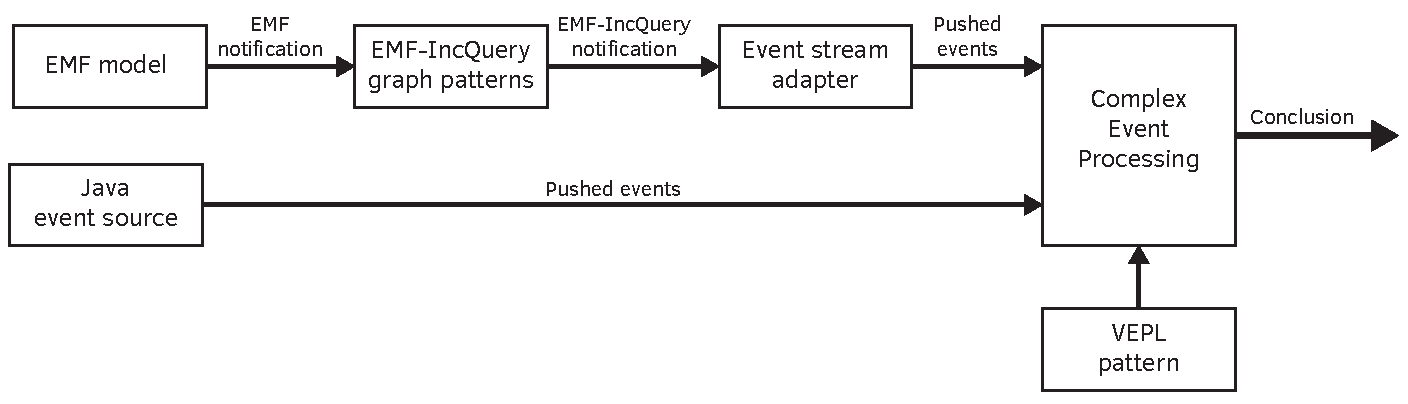
\includegraphics[width=0.9\linewidth]{figures/chapter_3/oldinput}
	\caption{A brief outline of the live model integration in VIATRA-CEP \redraw}
	\label{fig:viatracep:oldinputs}
\end{figure}

\tikzstyle{rect} = [
	thick,
	inner sep=2mm,
	%minimum width=30mm,
	minimum height=10mm,
	align=center,
	draw=black,
	rectangle
]

\usetikzlibrary{
	arrows,arrows.meta,
	shapes,shapes.geometric,shapes.misc,
	chains, trees,
	positioning,decorations.pathreplacing	
}
\begin{figure}[h]
\noindent
\makebox[\textwidth]{%

	\centering
	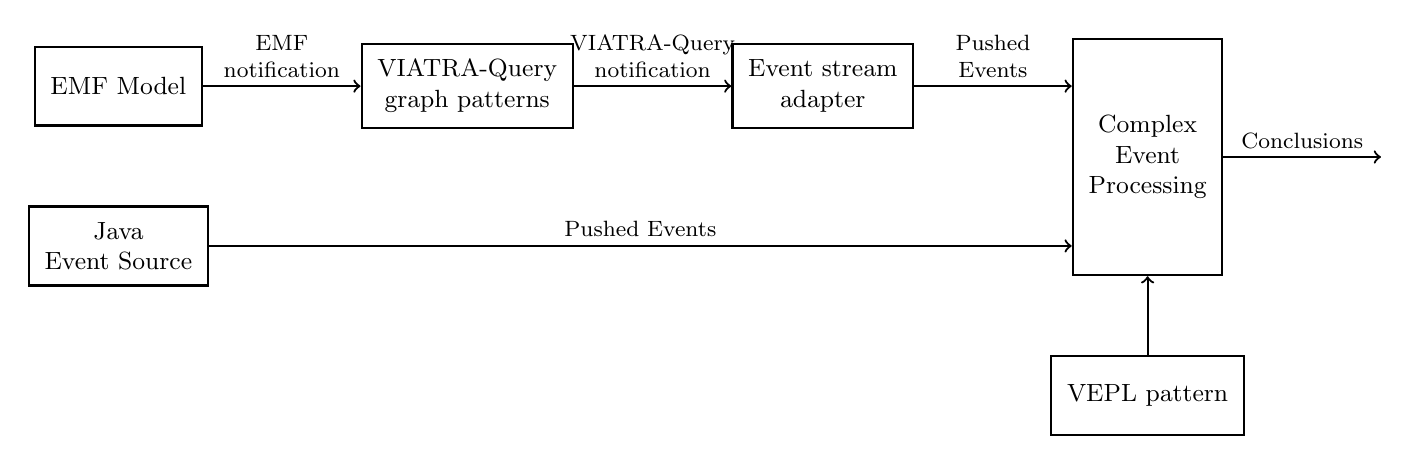
\begin{tikzpicture}[node distance=1cm and 2cm,
	edge/.style={thick, ->}
	]
	%
	\small{
	\node[rect, minimum height=30mm] (cep) {Complex\\Event\\Processing};
	\node[rect, left=of cep, yshift=9mm] (es) {Event stream\\adapter};
	\node[rect, left=of es] (vp) {VIATRA-Query\\graph patterns};
	\node[rect, left=of vp] (emf) {EMF Model};
	\node[rect, below=of emf] (jes) {Java\\Event Source};
	\node[rect, below=of cep] (vql) {VEPL pattern};
	\node[right=of cep] (fakeNode){};
	}
	%
	\footnotesize{
		\draw[edge](emf) -- (vp) node[midway, above, align=center]{EMF\\notification};
		\draw[edge](vp) -- (es) node[midway, above, align=center]{VIATRA-Query\\notification};
		\draw[edge](es) -- (es-|cep.west) node[midway, above, align=center]{Pushed\\Events};
		\draw[edge](jes) -- (jes-|cep.west) node[midway, above, align=center]{Pushed Events};
		\draw[edge](vql) -- (cep);
		\draw[edge](cep) -- (fakeNode) node[midway, above, align=center]{Conclusions};	
	}
	\end{tikzpicture}%	
}
\end{figure}%


\section{Event Pattern Language}
VIATRA-CEP uses a language called VIATRA Event Pattern Language (VEPL for short).
This language has intuitive syntax and the event patterns can be defined in
a very high level. 

\paragraph{Operators and semantics}
VEPL basic operators are shown in~\cref{tab:cep:veplop}.
There are additional operators, which can be considered syntactic sugars, shown in~\cref{tab:cep:veplsugar},
but these operators can be expressed with the basic operators as shown in~\cref{tab:cep:veplsugartobasic}, according to \citep{CEP}.

The semantics of the operators ``OR'' and ``AND'' are the following:
\begin{itemize}
	\item operator ``OR'' has a ``committed or'' semantic. This means if that one operand of the ``OR'' is not an atomic event, and that part starts a partial match, the other part of the ``OR'' is ignored while this part is active. \\
	E.g. if the pattern is $(A \rightarrow B)$ OR $C$,
	then trace $A,C$ will not match the pattern.\footnote{Meanwhile VEPL patterns are similar to patterns in regular expressions, they have different semantics. In case of a regular expression, pattern $(AB)|C$ , and the $A\,C$ trace would not cause a match. But since VEPL is used in the field of complex event processing, where an arbitrary prefix for all patterns is set by default, the equivalent of $(A \rightarrow B)$ OR $C$ is $\Sigma^\ast (AB)|C$}
	\item ``AND'' is a binary operator, e.g.~$A$ AND $B$ AND $C$ is equivalent to $(A$ AND $B)$ AND $C$,
	and it will not accept the trace $A\,C\,B$
\end{itemize}

\begin{table}
	\caption{Basic operators}		
	\label{tab:cep:veplop}
	\begin{tabularx}{\textwidth}{llX}
		\toprule
		Operator name &	Denotation & Meaning \\
		\midrule
		followed by & $p_1$ $\rightarrow$ $p_2$ & Both patterns have to appear in the specified order. \\
		or & $p_1$ OR $p_2$ &	One of the patterns has to appear. \\
		``infinite'' multiplicity & $p\{{\ast}\}$ & The pattern can appear 0 to infinite times. \\
		within timewindow &	$p[t]$ & Once the first element of the complex pattern $p$ is observed (i.e. the patterns ``starts to build up''), the rest of the pattern has to be observed within $t$ milliseconds. \\
		\bottomrule
	\end{tabularx}
\end{table}

\begin{table}
	\caption{Syntactic sugars}		
	\label{tab:cep:veplsugar}
	\begin{tabularx}{\textwidth}{llX}
		\toprule
		Operator name &	Denotation & Meaning \\
		\midrule
		and & $p_1$ AND $p_2$ & Both of the patterns has to appear, but the order does not matter.\\
		negation & NOT $p$ & On atomic pattern: event instance with the given type must not occur. On complex pattern: the pattern must not match. \\
		multiplicity & $p\{n\}$ & The pattern has to appear $n$ times, where n is a positive integer.\\
		``at least once'' multiplicity & $p\{+\}$ & The pattern has to appear at least once. \\
		\bottomrule
	\end{tabularx}
\end{table}

\begin{table}
	\caption{Syntactic sugars mapped to basic operators}		
	\label{tab:cep:veplsugartobasic}
	\begin{tabularx}{\textwidth}{llX}
		\toprule
		Operator name & Denotation & Equivalent \\
		\midrule
		and & $p_1$ AND $p_2$ & ($(p_1 \rightarrow p_2)$ OR $(p_2 \rightarrow p_1)$). \\
		negation & NOT $p$ & $\Sigma \setminus p$, where $\Sigma$ is the set of all the possible events. \mytodo{And complex NEG?} \\
		multiplicity & $p$\{n\} & $p \rightarrow p \rightarrow \dots p$, n times. \\
		``at least once'' multiplicity & $p$\{+\} & $p \rightarrow p\{\ast\}$ \\
		\bottomrule
	\end{tabularx}
\end{table}

\needspace{5cm}
\section{Contexts}

To define properties of execution of the pattern matching, the user can set which event context will be used for the execution.
These event contexts set the properties execution as of noise-reduction, and the maximal amount of partial matches at the same time.

\subsection{Matching and partial matches}
When a pattern is not matched yet, but the current trace is a possible prefix of the pattern, the trace will cause a partial match.
For example, if the pattern is $A \rightarrow B \rightarrow C$, and the trace is $A\,B$ then the pattern matcher only waits for an event $C$.
The event context defines the maximal amount of these partial matches.
For example, if there are multiple matches allowed at the same time, and the pattern is $A \rightarrow B$, the trace $A\,A\,B\,B$ will cause two matches, one at the reception of the first event of type $B$, and one after the reception of the second event of type $B$. 
If only one partial match would be used at the same time, the occurrence  first event of type $B$ would cause a match, but the second occurrence  would not.


\subsection{Noise and noise-reduction}
In most cases, where a Complex Event Processor is used, there are multiple event sources, with vast amount of event types.
Even in these cases, there are many pattern, which does not use all of these event types.
In VIATRA-CEP, the noise is defined as following: An incoming event, which will not increase the size of the currently non-contradictory postfix of the trace.
For example, if the pattern is $A \rightarrow B \rightarrow C$, and the previous trace is $A\,B$, an event $B$ is considered noise. Note that in this example, an event $A$ would not be noise, as it will either start a new partial match, if it is allowed, or restart the matching depending on the chosen context.

\subsection{Overview of the event contexts}

\begin{table}
	\caption{Event Contexts in VIATRA-CEP}		
	\label{tab:cep:contexts}
	\begin{tabularx}{\textwidth}{lcc}
		\toprule
		Context & Noise-reduction & Partial matches at the same time \\
		\midrule
		Strict Immediate & $-$ & Single \\
		Immediate & $-$ & Multiple \\
		Chronicle & $\checkmark$ & Multiple \\
		\bottomrule
	\end{tabularx}
\end{table}

All three different event contexts introduced in \citep{davidi} are shown in~\cref{tab:cep:contexts}.
These contexts can be defined separately for each event pattern, and they will define the execution semantics of the generated automata. 
An example of these contexts are shown on \cref{tab:cep:contextexample}. In this example the first three rows represent an example of the noise-reduction property, as the Chronicle Context ignores the events in the trace, which are not in the current pattern.
The last three rows represent an example of the multiple partial matches, as the Immediate and the Chronicle Event Contexts have two matches, while the Strict Immediate has only one.
The accepted parts of the traces are under- and overlined from their start to their end.


\begin{table}
	\caption{Examples of the Event Contexts in VIATRA-CEP}		
	\label{tab:cep:contextexample}
	\centering
	\begin{tabular}{@{}clcc@{}}
		\toprule
		VEPL pattern & Context & Trace & Accepted \\
		\midrule
		$A \rightarrow B$ & Strict Immediate & $A\,C\,B$ & $-$ \\[1ex]
		& Immediate & $A\,C\,B$ & $-$ \\[1ex ]
		& Chronicle & $\underline{A\,C\,B}$ & $\checkmark$ \\[4ex]
		%
		& Strict Immediate & $A\,\underline{A\,B}\,B$ & $\checkmark$ \\[1ex]
		& Immediate & $\mathrlap{\overline{\phantom{AAB}}} A\, \underline{A\,B\,B}$ & $2\times\checkmark$ \\[1ex]
		& Chronicle & $\mathrlap{\overline{\phantom{AAB}}} A\, \underline{A\,B\,B}$ & $2\times\checkmark$ \\[1ex]
		\bottomrule
	\end{tabular}
\end{table}



\section{Overview of the architecture}
In this section a short overview of the inside of the VIATRA-CEP is given.

The user first optionally defines the graph patterns on an EMF model, or simply defines atomic events.
Using these two, the user builds up complex event patterns, and sets the context for each event pattern. The event patterns are compiled to an automaton
whose execution semantics is defined by the context, as shown on \cref{fig:viatracep:oldcep}. 
Note that the overall semantics is defined by both the automaton generated from the event pattern, and the context.
If the goal is to create an extensible framework, one of the possible approaches is to use a general intermediate language. In this case additional languages only require a mapping to the intermediate language.
A well defined formal intermediate representation supports the formal verification of the CEP specification, and the semantics is desirable to be defined exclusively by the automaton.



\begin{figure}[h]
	\centering
	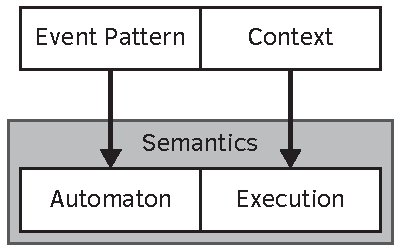
\includegraphics[width=0.4\linewidth]{figures/chapter_3/oldcep}
	\caption{The architectural overview of the VIATRA-CEP \redraw}
	\label{fig:viatracep:oldcep}
\end{figure}


\section{Intermediate modeling layer}
Our proposal is to use an intermediate language between the event pattern language and the automata representation, and to use this intermediate language as a common representation of the high level specification, as shown on \cref{fig:viatracep:newcep}. In addition, the long term goal is to support formal analysis of the defined properties. 


\begin{figure}[h]
	\centering
	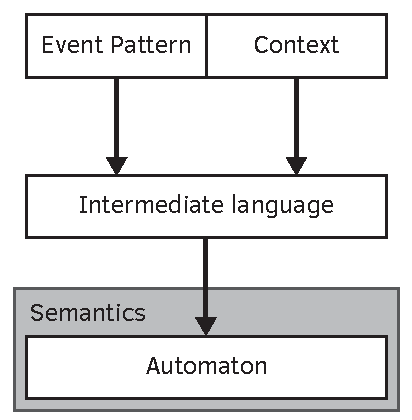
\includegraphics[width=0.4\linewidth]{figures/chapter_3/newcep}
	\caption{The architectural overview of our proposed architecture \redraw}
	\label{fig:viatracep:newcep}
\end{figure}


Using an intermediate language increases the extensibility of the framework, as additional pattern languages can be added later, by implementing a compiler from the high level language to the intermediate language, as shown on \cref{fig:viatracep:newinputs}.
The intermediate language would allow the user to combine patterns defined in multiple languages, as multiple automata could run and their simultaneous runs could be analysed in a formal way.


\begin{figure}[h]
	\centering
	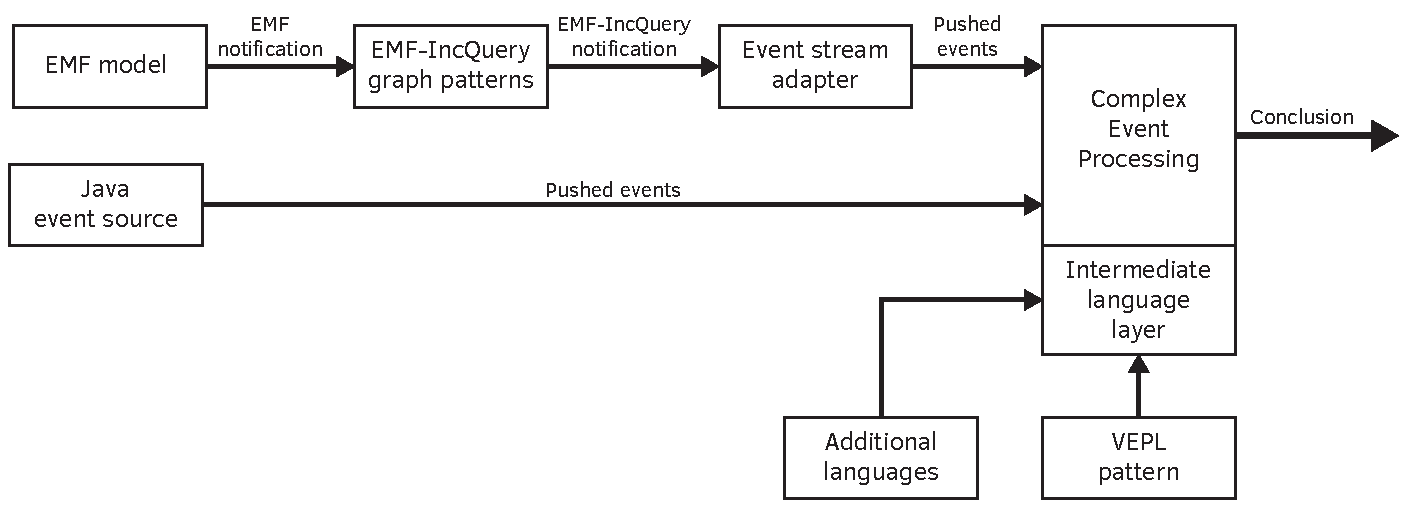
\includegraphics[width=0.9\linewidth]{figures/chapter_3/newinput}
	\caption{A brief outline of the live model integration in VIATRA-CEP, with the intermediate language \redraw}
	\label{fig:viatracep:newinputs}
\end{figure}
	\chapter{Intermediate Language}
	\label{chap:cep}
	
	\todo{Check the chapter for mixing Timeout and timed!}
	
	Regular languages are widely used in computer science as they can be represented efficiently by finite state machines.		
	In our research according to \citep{davidi} I found out, that using regular expressions with timing extensions and parameters we are able to express the temporal patterns of VIATRA-CEP.
	Since regular expressions are widely used by the engineers and finite state automata provide clear semantics they are a good candidate as an intermediate language.
	
	First we overview formalisms from the literature, and suggest parametric timed region automaton as an intermediate formalism.
	As many of the high level specification languages like VEPL and Sequence charts can be characterized with the help of regular languages,
	this was the motivation behind our research.% Our findings are based on \citep{dicep}.
	
	We are going to introduce every step through an example: 
	We will specify a runtime verification component (also known as monitor) which will be in accepting state if the system is violating the rules of the two phase lock algorithm extended with a timeout.
	This can be considered as a runtime verification component of such system. This example is based on the File System example of paper \citep{marq}.
	
	In the two phase locking algorithm there are three rules to be held :
	\begin{enumerate}
		\item Resources must be allocated in a previously defined sequence (this sequence is the same for all tasks).
		\item If a task releases a resource, it is not allowed to do any more allocations.
		\item The first phase must finish after 10 seconds, i.e.~the time between the first allocation and the first release must be less than 10 seconds\footnote{We could use a better example such as ``A resource can not be in allocated state for more than 10 sec'', but this would make the example really complex.}. 
	\end{enumerate}
	
	Since this example uses resources, their behavior is defined as following:
	Each resource can be allocated once before every release, and can be released once before every allocation.
		
	\section{Overview of Formalisms}

	\begin{figure}[h]
			\begin{tikzpicture}[ edge/.style={thick, ->}]
			\small{
				\matrix (m) [matrix of nodes, nodes={rect,text width=0.2\linewidth, anchor=center 
				,  minimum height=4.25em}, row sep=3em, column sep=5em]
				{
					Regular\linebreak{}Expression &  Timed Regular Expression & Parametric Timed Regular Expression \\
					Nondeterministic Event Automaton &  Nondeterministic Timeout Region Event Automaton &  Parametric Timeout Region Event Automaton \\
					 Deterministic Event Automaton & Nondeterministic Timeout Event Automaton &  Parametric Timeout Event Automaton \\
				};
			}
			\footnotesize{
			\draw[edge](m-1-1) -- (m-1-2) node[midway, above, align=center]{+timing};
			\draw[edge](m-1-2) -- (m-1-3) node[midway, above, align=center]{+parameters};
			%
			\draw[edge](m-2-1) -- (m-2-2) node[midway, above, align=center]{+timing};
			\draw[edge](m-2-1.south east) -- (m-3-2.north west) node[midway, above, sloped, align=center]{+timing};
			%
			\draw[edge] (m-2-2) -- (m-2-3)  node[midway, above, align=center]{+parameters};
			\draw[edge] (m-3-2) -- (m-3-3) node[midway, above, align=center]{+parameters};
			%
			\draw[edge] (m-1-1) -- (m-2-1)  node[midway, right, align=center]{transformation};
			\draw[edge] (m-2-1) -- (m-3-1) node[midway, right, align=center]{transformation};
			%
			\draw[edge] (m-1-2) -- (m-2-2) node[midway, right, align=center]{transformation};
			\draw[edge] (m-2-2) -- (m-3-2) node[midway, right, align=center]{transformation};
			%
			\draw[edge] (m-1-3) -- (m-2-3) node[midway, right, align=center]{transformation};
			\draw[edge] (m-2-3) -- (m-3-3) node[midway, right, align=center]{transformation};
			}
			\end{tikzpicture}
		\caption{Overview of the formalisms }
		\label{fig:cep:folyamatabra}
	
	\end{figure}%
	
	The used formalisms and their relations are show on \cref{fig:cep:folyamatabra}.
	The vertical arrows show that for each regular expression an automaton can be constructed with a transformation, which accepts the language specified with the regular expression.
	The horizontal arrows show that each formalism can be extended with the required properties; timing and parameters respectively.
	Note that even the Deterministic Event Automaton could be extended with Timing, and a formalism could be constructed for it, however there are no known algorithms to construct a Deterministic Timed Automaton.
		
	\section{Regular Languages}
	
		Regular Languages are commonly used both in the industry and in the academic researches as they commonly serve as a domain specific language.
		Most of their properties which are interesting from the academic point of view can be analyzed and decided, and they are simple enough to be used in industrial projects to ease up the description of something which does not require a more complex language.
	
		\subsection{Regular Expression}
		
			In this particular example, we need a language to describe event sequences. To do so, one of the most common formalism is regular expressions, where the alphabet $\Sigma$ is the set of possible events.
	
			
			\begin{dfn}
				\label{dfn:cep:re}
				Regular Expressions over an alphabet $\Sigma$ (also referred to as $\Sigma$-expressions)
				are defined using the following families of rules.
				\begin{enumerate}
					\item $a$ for every letter $a \in \Sigma$ and the special symbol $\varepsilon$ are expressions.
					\item If $\varphi, \varphi_1, \varphi_2$ are $\Sigma$-expressions then %
						$ %
						\varphi_1 \varphi_2,
						\varphi_1 | \varphi_2,
						\varphi^\ast
						$ are $\Sigma$-expressions\citep{tre}.
				\end{enumerate}
			\end{dfn}
	
			The meaning of these operators:
			\begin{itemize}
				\item $\varphi_1 \varphi_2$: Sequence, $\varphi_2$ must occur after $\varphi_1$.
				\item $\varphi_1 | \varphi_2$: Choice, $\varphi_1$ or $\varphi_2$ must happen.
				\item $\varphi^\ast$: Closure (also known as Kleene-star), $\varphi$ can occur $n$ times, where $0 \leq n < \infty$
			\end{itemize}
			
	
			To illustrate the usage of the regular expressions in the two phase locking example, the behavior ``After a task has released a resource, it's not allowed to allocate again'' is described with the regular expression : $a \; (a)^* \; r \; (r)^* \; a $, where $a$ is short for allocation and $r$ is short for release.
	
	
		\subsection{Deterministic Finite Event Automaton}
			To accept regular expressions, the most common solution is to construct an automaton accepting the language generated by the regular expressions. Various  algorithms exist for the generation of deterministic finite automaton from regular expressions. \todo{Cite?}
			
			\begin{dfn}
				\label{dfn:cep:ea}
				A Deterministic Finite Event Automaton is a tuple $\langle Q,\Sigma,\delta,q_0, F \rangle$\citep{lam2006compilers} where: 
					\begin{itemize}
						\item $Q$ is a finite, nonempty set, representing the states of the automaton,
						\item $\Sigma$ is a finite, nonempty set, representing the event set of the automaton,
						\item $\delta$ is a subset of tuples $\langle Q \times \Sigma \times Q \rangle$,
							and the number of outgoing edges from each state for each event is only one 
							i.e.~$\forall s_0 \in Q$ and $\forall e_0 \in \Sigma$ : $|\langle s_0, e_0, s_1 \rangle| = 1$, where $s_1 \in Q$. Nondeterminism is not allowed,
						\item $q_0 \in Q$ the initial state,
						\item $F \subseteq Q$ the set of the accepting states.
					\end{itemize}	
			\end{dfn}
		
			\begin{dfn}
				\label{dfn:cep:ea:inputseq}
				An input sequence for a Deterministic Finite Automaton is $(e_1, e_2, \dots, e_n )$, where $\forall i : e_i \in \Sigma$, i.e.~a sequence of events.
			\end{dfn}
		
			\begin{dfn}
				\label{dfn:cep:ea:trace}
				A trace in an Deterministic Event Automaton is
				a sequence of states $(r_0, r_1, \dots, r_m)$, where $\forall i: r_i \in Q$,
				for the input sequence $(e_1, e_2, \dots, e_n)$ if:
				\begin{itemize}
					\item $r_0 = q_0$, i.e.~the first state of the trace is the initial state of the Automaton,
					\item If the automaton has a trace $(r_0,\dots,r_{i-1})$ for input sequence $(e_1,\dots,e_{j-1})$ then either
					\begin{itemize} 
						\item $\langle r_{i-1}, \varepsilon, r_i \rangle \in \delta$, or
						\item  $\langle r_{i-1}, e_j, r_i \rangle \in \delta$ is true,
					\end{itemize}
					\item the last $r_m$ state is reached by reading event $e_n$ (Or more precisely the after reading the last event $r_m$ is reachable using only
					$\varepsilon$-transitions)
				\end{itemize}
				A trace is accepting if $r_n \in F$.
			\end{dfn}
		
			\begin{dfn}
				\label{dfn:cep:ea:accepting}
				An event automaton accepts an input sequence if exists an accepting trace for the input sequence.
			\end{dfn}
		
			\begin{dfn}
				\label{dfn:cep:ea:token}
				A token in a Nondeterministic Finite Event Automaton a set of the active states.
			\end{dfn}
			
			Just to illustrate the operation of the Finite Automata we can use a token assigned to the active state.
	
			The semantics is illustrated as follows. 
			\begin{itemize}
				\item At initialization the token is at the initial state $f_0$.
				\item When receiving input $e$, where $e \in \Sigma$, if the token is on state $s$ the next state will be $s'$ where
				$\delta \langle s,e,s' \rangle$.% For short, from now the notation $s \rightarrow s'$ will be used. 
				\item If the token enters state $s'$ where $s' \in F$ then the input sequence is accepted. 			
			\end{itemize}
	
	
			The regular expression of the example can be compiled to the event automaton of~\cref{fig:cep:fa}. 
	
			Note that the automaton only accepts the incorrect traces as our complex event processing framework allows to define reactions when the automaton enters an acceptor state.
			
				
				\begin{figure}[h]
					\centering
					\begin{tikzpicture}[
					edge/.style={
						->
					},
					every loop/.style={
						looseness=2,
						min distance = 2cm,
						in = -120,
						out = -60
					}
					]
					\node[elliptic state, initial, align = center] (initial) {initial\\state};
					\node[elliptic state, right=of initial, align = center] (alloc) {allocating\\phase};
					\node[elliptic state, right=of alloc, align = center] (release) {releasing\\phase};
					\node[elliptic state, accepting, right=of release, align = center] (error) {error\\state};
					
					\path[->]
					(initial) edge[bend left = 45] node[above] {$a$}  (alloc)
					(alloc) edge[bend left = 45] node[above]{$r$} (release)
					(release) edge[bend left = 45] node[above] {$a$} (error)
%					
					(alloc) edge[loop below] node{$a$} ()
					(release) edge[loop below] node{$r$} ();
					
					\end{tikzpicture}
					\caption{Event automaton of the two phase locking example}
					\label{fig:cep:fa}
				\end{figure}

			

		\subsection{Nondeterministic Finite Event Automaton}
		
		\begin{dfn}	
			\label{dfn:cep:nea}
			A Nondeterministic Finite Event Automaton is a tuple $\langle Q,\Sigma',\delta,q_0, F \rangle$, where:
			\begin{itemize}
				\item $Q, q_0$, and $F$ are the same as in \cref{dfn:cep:ea},
				\item $\Sigma'$ is $\Sigma \cup \varepsilon$, where $\Sigma$ is the same as in \cref{dfn:cep:ea}
				\item $\delta$ is a subset of tuples $\langle Q \times \Sigma' \times Q \rangle$.
				Note that there could be more than one transition for one state with the same event.
			\end{itemize}
		\end{dfn}
	
		\begin{dfn}
			\label{dfn:cep:nea:trace}
			A trace in an Deterministic Event Automaton is
			a sequence of states $(r_0, r_1, \dots, r_n)$, where $\forall i: r_i \in Q$,
			for the input sequence $(e_1, e_2, \dots, e_n)$ if:
			\begin{itemize}
				\item$r_0 = q_0$, i.e.~the first state of the trace is the initial state of the Automaton,
				\item $\forall i \in (1,\dots,n-1): \langle r_i, e_{i+1}, r_{i+1} \rangle \in \delta$ i.e.~exists a transition between state $r_i$ and $r_{i+1}$ with the label of the $e_{i+1}$ according event.	
				\item The last $r_n$ is reached after reading the entire input sequence.	
			\end{itemize}
			A trace is accepting if $r_n \in F$.
		\end{dfn}
			
		\begin{dfn}
			\label{dfn:cep:nea:accepting}
			An event automaton accepts an input sequence if exists an accepting trace for the input sequence.
		\end{dfn}
		
		\begin{dfn}
			\label{dfn:cep:nea:token}
			A token in a Deterministic Finite Event Automaton is the active state.
		\end{dfn}
		
		\subsection{Transformation from Regular Expression to Deterministic Finite Automaton}
			The transformation of simple (not timed and parametric) regular expressions are well known in the current literature. The various algorithms were investigated and a chosen algorithm from \citep{lam2006compilers} is implemented.
	
			
			\subsubsection{Transformation from Regular Expression to Nondeterministic Automaton with $\bm{\varepsilon}$ transitions}
			\label{section:re2nfa}
			First the regular expression is transformed to a nondeterministic automaton with recursive rules for each operator
			\begin{itemize}
				\item The automaton corresponds to a simple event is constructed as an initial state and an acceptor state with one transition between them, which has the label of the event, as shown on \cref{fig:cep:nfaevent}. Note that this is the only non-recursive rule, as the concrete syntax tree's leaves are always Events, therefore this is where the recursion always stops.\todo{There is a better terminology for ``algorithm stops'' :D}
				\item The sequence of two expressions are compiled in two steps, first the two subexpressions are compiled into one automaton each. After that we merge the acceptors states of the first automaton with the initial state of the second automaton, i.e.~remove the acceptor flag from the first automaton's acceptor states, and add every outgoing transition of the second automaton's initial state to the first automatons acceptor states, as shown on \cref{fig:cep:nfasequence}
				\item A choice can be compiled in two steps. First the two subexpressions are compiled into one automaton each. In the second step we create one new initial state, and create a two $\varepsilon$-transition from the new initial state to the two subexpression's compiled automata's initial state. After that we create one $\varepsilon$-transition from their acceptor states to a newly created acceptor state. The result's initial state will be the newly created state and the result's only acceptor state will be the newly created one, as shown on \cref{fig:cep:nfachoice}
				\item A closure can also be compiled in two steps, first the internal expression has to be compiled to the automaton and a new initial and acceptor state has to be constructed. Then four $\varepsilon$ transition needs to be added:
				\begin{enumerate}
					\item From the compiled automaton's acceptor state to it's initial state,
					\item From the new initial state to the subexpression's initial state,
					\item From the subexpression's acceptor state to the new acceptor state,
					\item From the new initial state to the new acceptor state.
				\end{enumerate}
			\end{itemize}
		
			\todo{Missing the AND, probably just don't tell the reader about it?}
			
			\begin{figure}[h]
				\centering
				\begin{tikzpicture}[
				node distance=1cm and 2cm,
				edge/.style={->}
				]
					\node[state,initial] (initial) {$i$};
					\node[state,accepting, right=of initial] (final) {$f$};
					\draw[edge](initial) -- (final) node[midway, above, align=center]{$a$};
				\end{tikzpicture}
				\caption{Constructed NFA from the simple event $a$}
				\label{fig:cep:nfaevent}
			\end{figure}
		
			\begin{figure}[h]
				\centering
				\begin{tikzpicture}[
					edge/.style={->}
					]
					\node[state] (initial) {$i$};
					\node[right=of initial] (nt) {$N(t)$};
					\node[state, right=of nt] (common) {};
					\node[right=of common] (ns) {$N(s)$};
					\node[state,accepting, right=of ns] (final) {$f$};
					\node[draw, ellipse, initial, inner xsep=-3mm, fit=(initial) (nt) (common)] (left elipsis) {};
					\node[draw, ellipse, inner xsep=-3mm, fit=(common) (ns) (final)] (right elipsis) {};
				\end{tikzpicture}
				\caption{Constructed NFA from the sequence $N(s)\;N(t)$}
				\label{fig:cep:nfasequence}
			\end{figure}
			
			\begin{figure}[h]
			\centering
			\begin{tikzpicture}[
				edge/.style={->}
				]
				\node[state, initial] (initial) {$i$};
				%
				\node[state, above right=of initial] (nti) {};
				\node[right=of nti] (nt) {$N(t)$};
				\node[state, right=of nt] (ntf) {};
				\node[draw, ellipse, inner xsep=-3mm, fit = (nti) (nt) (ntf)] {};
				%
				\node[state, below right=of initial] (nsi) {};
				\node[right=of nsi] (ns) {$N(s)$};
				\node[state, right=of ns] (nsf) {};
				\node[draw, ellipse, inner xsep=-3mm, fit = (nsi) (ns) (nsf)] {};
				
				\node[state, accepting, above right=of nsf] (final) {$f$};
				
				\draw[edge] (initial) -- (nti) node[midway, above, sloped, align=center]{$\varepsilon$};
				\draw[edge] (initial) -- (nsi) node[midway, above, sloped, align=center]{$\varepsilon$};
				
				\draw[edge] (ntf) -- (final) node[midway, above, sloped, align=center]{$\varepsilon$};
				\draw[edge] (nsf) -- (final) node[midway, above, sloped, align=center]{$\varepsilon$};
				
			\end{tikzpicture}
			\caption{Constructed NFA from the choice $N(s)|N(t)$}
			\label{fig:cep:nfachoice}
		\end{figure}
			
			\begin{figure}[h]
				\centering
				\begin{tikzpicture}[
				edge/.style={->}, auto
				]
				\node[state, initial] (initial) {$i$};
				%
				\node[state, right=of initial] (nsi) {};
				\node[right=of nsi] (ns) {$N(s)$};
				\node[state, right=of ns] (nsf) {};
				\node[draw, ellipse, inner xsep=-3mm, fit = (nsi) (ns) (nsf)] {};
				%
				\node[state, accepting, right=of nsf] (final) {$f$};
				\path[->]
				(initial) edge node[near start] {$\varepsilon$}  (nsi)
				(nsf)     edge node[near end] {$\varepsilon$}                (final)  
				(nsf)     edge[bend left = 75] node {$\varepsilon$} (nsi)    
				(initial) edge[bend left = 60]  node {$\varepsilon$} (final) ;
				
				\end{tikzpicture}
				\caption{Constructed NFA from the closure $N(s)^*$}
				\label{fig:cep:nfasterisk}
			\end{figure}
			
	
			\subsubsection{Transformation from Nondeterministic Automaton to Deterministic Automaton}
			
					\begin{algorithm}
				\SetAlgoLined
				\SetKwInOut{Input}{input}\SetKwInOut{Output}{output}
				\Input{An NFA $N$}
				\Output{A DFA $D$ accepting the same language as $N$}
				initially, $\varepsilon$-closure($s_0$) is the only state in $\mathit{Dstates}$, and it is unmarked\;
				\While{there is an unmarked state $T$ in $\mathit{Dstates}$}{
					mark $T$\;
					\ForEach{input symbol $a$}{
						$U = $ $\varepsilon$-closure(move($T,a$))\;
						\If{$U$ is not in $\mathit{Dstates}$}{
							Add $U$ as an unmarked state to $\mathit{Dstates}$\;
						}
						$\mathit{Dtran}[T,a] = U$ \;
					}
				}
				\caption{The subset construction of a DFA from an NFA}
				\label{alg:cep:subset}
			\end{algorithm}
			
			\begin{algorithm}
				\SetAlgoLined
				\SetKwInOut{Input}{input}\SetKwInOut{Output}{output}
				\Input{A set of states $T$}
				\Output{A set of states $\varepsilon$-closure($T$)}
				push all states of $T$ onto $\mathit{stack}$\;
				initialize $\varepsilon$-closure($T$) to $T$\;
				\While{$\mathit{stack}$ is not empty}{
					pop $t$ from the $\mathit{stack}$ \;
					\ForEach{state $u$ with an edge from $t$ to $u$ labeled $\varepsilon$}{
						\If{$u$ is not in $\varepsilon$-closure($T$)}{
							Add $u$ to $\varepsilon$-closure($T$)\;
							push $u$ onto $\mathit{stack}$ \;
						}
					}
				}
				\caption{Computing $\varepsilon$-closure($T$)}
				\label{alg:cep:eclosure}
			\end{algorithm}
			
			The algorithm is introduced on \cref{alg:cep:subset}.
			The algorithm constructs a transition table $\mathit{Dtran}$ for $D$. Each state of $D$ is a set of NFA states, and we construct $\mathit{Dtran}$ so $D$ will simulate ``in parallel'' all possible moves $N$ can make on a given input trace. Our first problem is to deal with $\varepsilon$-transitions of $N$ properly.
	
			Move($T,a$) is the set of states of the NFA which there is a transition on input symbol $a$ from some state in $T$.
			
			The algorithm for calculating the $\varepsilon$-closure is shown on \cref{alg:cep:eclosure}.
			
		\section{Timed Regular Languages}	
		
		Timed Regular Languages are an extension over the Regular Languages to express timed properties.
		These timed properties are common in most of the usecases as many system has timed behavior which can be described using Timed Regular Languages.
		
			\subsection{Timeout Regular Expression}
		
			Using the previously defined semantics timed properties can not be expressed, but regular expressions can be extended to a formalism which can do so: the timeout regular expressions.
			
			\begin{dfn}
				\label{dfn:cep:tre}
				Timeout Regular Expressions over an alphabet $\Sigma$ (also referred to as $\Sigma$-expressions)
				are defined using the following rules.
				\begin{enumerate}
					\item $a$ for every letter $a \in \Sigma$ and the special symbol $\varepsilon$ are expressions.
					\item If $\varphi, \varphi_1, \varphi_2$ are $\Sigma$-expressions then %
						$ %
						\varphi_1 \; \varphi_2,
						\varphi_1 | \varphi_2,
						\varphi^\ast,$ and 
						$\langle \varphi \rangle_I$, 
						are $\Sigma$-expressions, where $I$ is an positive real number for timeout. % \citep{tre}
				\end{enumerate}
			\end{dfn}
	
	
			The new operator is $\langle \varphi \rangle_I$ which means, that the whole $\varphi$ has to be observed within the given time.	
			The implementation and algorithmization with intervals instead of timeouts as in \citep{tre} are considered future work.
	
			With the timed regular expression formalism the example can be extended with timing, and adding the concept timeout becomes possible.
			The new expression will be: $ \langle a \; (a)^\ast \rangle_{t > 10} \; r \; (r)^\ast \; a$
			
			\subsection{Timeout Region Automaton}
			
			Timeout Region Automaton is introduced as an intermediate step between the Timeout Regular Expression and the Timeout Automaton as it is a step closer to the regular expression.
			However the Timeout Region Automaton has the same expressive power as the Timeout Regular Expression the more general and better known Timeout Automaton is more expressive.
			If in the future for some use cases the Regular Expression lacks the required expressiveness then the Timeout Automata can be used as an intermediate language as well.
			
			We add a syntactic sugar to ease the compilation of high level languages to this intermediate language.
			Using timed regions in our automaton language has the same motivation as the application of regions in state chart formalisms.
			
			From now on, the notation $\mathit{Reg}$ will be used for regions, which is a set of states, i.e.~$\mathit{Reg}~\subseteq~Q$
			
			
			\begin{dfn}
				\label{dfn:cep:trea}
				A Timeout Region Event Automaton is a tuple $\langle Q,\Sigma,\delta,q_0, F, t, T \rangle$ where
				\begin{itemize}
					\item $Q, q_0,$and $F$ are the same as in \cref{dfn:cep:nea},
					\item $\Sigma$ is the same as $\Sigma'$ in \cref{dfn:cep:nea}, 
					
					\item $T$ is a set of tuples $\langle \mathit{Reg}, \RR \rangle$ i.e.~a set of timeout clock variables for a set of states,
					\item and $\delta$ is the union of discrete and timed transitions i.e.~$\delta_t \cup \delta_d$ where
					\begin{itemize}
						\item $\delta_d$ is the same as $\delta$ in \cref{dfn:cep:nea},
						\item and $\delta_t$ represents timed transitions and defined as the set of tuples $\langle \mathit{Reg} , \mathbb{R} , Q \rangle$, i.e.~a tuple which represents a timed region, the value of the maximum time elapsed
					\end{itemize}
					
				\end{itemize}
			\end{dfn}
			
	%		WTF: \linebreak the set of which have outgoing timed transitions i.e.~$ \forall R_i \in \mathit{Reg}, \exists t, \exists q  \subseteq \delta_t \langle R_i, t, q \rangle$ 
			
			The semantics of the timed region automaton is defined as follows:
			$Q_t \subseteq Q$ is the set of states with outgoing timed transitions, 
			i.e.~$\forall q \in Q_t$ : $ q \in R $. 
			
			
			Let us use the following notations: 
			
			\begin{itemize}
				\item $s$ is the currently active state, and $s'$ is the next state according to $\delta$.		
				\item $r$ is the set of currently active regions, i.e.~$r \subseteq \mathit{Reg}$ where $\exists r_s : r_s \in r, s \in r_s $ 
				\item $r'$ is the set of regions the token enters, i.e.~$r \subseteq \mathit{Reg}$ where $\exists r_s :  r_s \in r, s' \in r_s $ 
				\item $r^+ \subseteq \mathit{Reg}$ is a set of timed regions the token has just entered, i.e.~$r^+ = r' \setminus r$ 
				\item $r^- \subseteq \mathit{Reg}$ is a set of timed regions the toke has just left i.e.~$r^- = r \setminus r'$
			\end{itemize}
			
			Rules  have to defined for the initialization of the automaton, entering states with timed outgoing transitions and we also define the general rules of changing states. 
			
			\begin{enumerate}
				\item Initialization Rule : At the initialization  of the automaton, we have to set all clock variables to $\infty$ 
				i.e.~$\forall t_i, \forall q_i, T \langle r_i, t_i \rangle, t_i \coloneqq \infty $, where $r_i \in R$
				
				\item Entering new timed region rule :
				If a token enters a new set of timed regions, 
				i.e.~$r^+ \neq \emptyset$, 
				the timers are set according to the timeouts, 
				i.e.~$\forall t_{\textit{timeout}} : t_{\textit{timeout}} \coloneqq t + t_i $ where $ r_t \in r^+, \exists q ,\delta_t\langle  r_t,t_i,q \rangle, T \langle r_t, t_{\textit{timeout}} \rangle$
				
				\item Firing Transition Rule: Choose an enabled transition from the set of enabled discrete or timed transitions. 
				There are two cases, the chosen transition is:
				\begin{enumerate}
					\item Discrete Transition: In case of $r^- = \emptyset$ than the execution of the transition is as in described formerly. 
					If the token exits a region i.e.~$r^- \neq \emptyset$, 
					then the following rule extends the firing rule of discrete transitions:
					$\forall t_s, \forall q_s$ in $ \delta_t \langle r_i, t_s, q_s \rangle$ where $r_i \in r^-$, the timer of the regions are invalidated i.e.~	$t_s \coloneqq \infty$
					\item Timed Transition: The transition with the minimal timeout value is selected, 
					i.e.~transition $\exists t_i, \exists s_i, \delta_t \langle r_i, t_i, s_i \rangle$ where $ r_i \in r$ and $t_{\textit{min}}$ is the minimum from all $t_i$,
					than the following rules apply:
					the global time is set $t \coloneqq t_{\textit{min}}$, 
					the local clocks the token just left are invalidated i.e.~
					$\forall t_s, \forall q_s$ in $ \delta_t \langle r_i, t_s, q_s \rangle$ where $r_i \in r^-$, the timer of the regions are invalidated i.e.~$t_s \coloneqq \infty$ 
					and move to the next state according to $\delta_t$.
				\end{enumerate}			
			\end{enumerate}
			
			
			We can generate from the expression % $(a (a)^\ast r (r)^\ast a)|( \langle a (a)^\ast r \rangle_{t < 10 s})$
			$(\langle a (a)^\ast \rangle_{t > 10} r (r)^\ast a)$
			the automaton of~\cref{fig:cep:trea}.
			Note the additional timed region which contains the ``allocating phase'' state.
			
			\begin{figure}[h]
				\centering
				\begin{tikzpicture}[
				edge/.style={
					->
				},
				every loop/.style={
					looseness=2,
					min distance = 15mm,
					in = -120,
					out = -60
				}
				]
				\node[elliptic state, initial, align = center] (initial) {initial\\state};
				\node[elliptic state, right=of initial, align = center] (alloc) {allocating\\phase};
				\node[below = of alloc, align = right, minimum width=0.15\linewidth, yshift=-7.5mm] (fake below) {};
				\node[elliptic state, right=of alloc, align = center] (release) {releasing\\phase};
				\node[elliptic state, accepting, right=of release, align = center] (error) {error\\state};
				
				\node[draw, rect, fit = (fake below) (alloc)
%				, inner xsep = 0mm
				] (timing) {};
				
				\node [rect, minimum height=0mm ,anchor=south east] at (timing.south east) { $t < 10$};
				
				\path[->]
				(initial) edge[bend left = 45] node[above] {$a$}  (alloc)
				(alloc) edge[bend left = 45] node[above]{$r$} (release)
				(release) edge[bend left = 45] node[above] {$a$} (error)
				%					
				(alloc) edge[loop below] node{$a$} ()
				(release) edge[loop below] node{$r$} ();
				%
				\draw [->] (timing.south east) to [out=0,in=-90] (error);
				
				\end{tikzpicture}
				\caption{Timed region event automaton of the two phase locking example}
				\label{fig:cep:trea}
			\end{figure}
		
			
			\subsection{Nondeterministic Timeout Event Automaton}
			
				For accepting languages generated by timed regular expressions, the concept of timed event automaton is introduced.	
				\todo{lost reference on \citep{alur1994theory}.}
				
				\begin{dfn}
					\label{dfn:cep:tea}
					A Nondeterministic Timeout Event Automaton is a tuple $\langle Q,\Sigma,\delta,q_0, F, C \rangle$ where
					\begin{itemize}
						\item $Q, \Sigma, q_0,$ and $F$ are the same as in \cref{dfn:cep:trea},	
						\item $C$ is a finite set of clocks.
						\item $\delta \subseteq \langle Q \times \Sigma' \times Q \times (\RR^+ \cup \{\infty\})^C \times 2^C \rangle$ i.e.~the transitions of the system in the order of:
							the state which is the source of the transition,
							the corresponding event for the transition (or $\varepsilon$ if it is an $\varepsilon$-transition),
							the state which is the destination of the transition,
							a function which assigns time values for each clock,
							and the set of clocks which needs to be reset upon firing the transition.
					\end{itemize}
				\end{dfn}
			
				\begin{dfn}
					\label{dfn:cep:tea:inputseq}
					A timed input sequence is denoted $(e_0, t_1, e_1, \dots, t_n, e_n)$ where $e_i \in \Sigma'$ and $t_i \in \RR^+_0$ i.e.~ a sequence of events and the elapsed times between them.
				\end{dfn}
			
				\begin{dfn}
				\label{dfn:cep:tea:trace}
				A trace in a Timeout Event Automaton is a sequence described as
				$(r_0, \langle a_1, t_1, v_1\rangle, \dots, \langle a_n, t_n, v_n \rangle, r_n)$, where $\forall r_i \in Q, \forall a_i \in \Sigma', \forall t_i \in \RR^+$ i.e.~a sequence of states, the elapsed time between them, and the clock assignments. The trace corresponds to to the timed input sequence $(e_0, t_1, e_1, \dots, t_n, e_n)$ if:
				\begin{itemize}
					\item $r_0 = q_0$, i.e.~the first state of the trace is the initial state of the Automaton,
					\item $\forall i \in [1,n - 1] \colon \langle r_i, a_{i+1}, r_{i+1}, u, \mathit{Res} \rangle \in \delta$,
						${v_i}' = v_i + t_{i+1}$, $\forall c \in C \colon {v_i}'(c) < u(c)$, and
						$$v_{i+1} = \begin{cases}
										0      & \text{if\ } c \in    \mathit{Res} \\
										{v_i}' & \text{if\ } c \notin \mathit{Res}
									\end{cases}$$
					\item The last $r_n$ is reached after reading the entire input sequence.	
				\end{itemize}
				A trace is accepting if $r_n \in F$.
				\end{dfn}
				
				\begin{dfn}
					\label{dfn:cep:tea:accepting}
					A Nondeterministic Timeout Event Automaton accepts a timed input sequence if exists an accepting trace for the timed input sequence.
				\end{dfn}
				
				\begin{dfn}
					\label{dfn:cep:tea:token}
					A token in a Nondeterministic Timeout Event Automaton is a set of the active states with their timer values.
				\end{dfn}
				
				The semantics of the timed deterministic finite automaton is defined as follows:
				
				\todo{Revision required}
				
				$Q_t \subseteq Q$ is the set of states with outgoing timed transitions, 
				i.e.~$\forall s \in Q_t$ : $ \exists t, t \in \delta \colon t = \langle s, a, s', h, c \rangle$, where $a \in \Sigma$, $s' \in Q$, $h \neq \emptyset$, and $c \neq \emptyset$.
				
				We have to define rules for entering states with timed outgoing transitions and we also define the general rules of changing states. 
				The current tokens in the automaton are noted as $\tau_{act}$.
				
				\begin{enumerate}
					\item Initialization rule: 
						$\forall c \in C \colon c \coloneqq \infty$, i.e.~on initialization of the automaton, all timeout clocks must be invalidated.
						On initialization a token must be placed on the initial state of the automaton.
					\item Firing Transitions Rule:
						$Q_{act}$ is the set of states which contains tokens.
						Upon receiving input $i$, where $i \in \Sigma$, $\forall q \in Q_{act}$, $\forall t \in \delta \colon \delta \langle q, i, q', T, \mathit{Res} \rangle$,
						$\forall c \in \mathit{Res} \colon c \coloneqq \infty$,
						$\forall c \in C \colon c \coloneqq T(c)$,
						the token is copied from $q$ to $q'$.
						The old tokens which are not created in this step must be removed.
					\item Timeout Rule:
						If one of the clocks reaches 0 for a token, the computation fails, and the token must be removed.
				\end{enumerate}
	
		\subsection{Transformation from Timed Regular Expressions to Timed Automata}
			\label{section:tre2tnfa}	
			Constructing a Timeout Region Automaton from a Timeout Regular expression depends on the steps described in \cref{section:re2nfa} as only one new operator has been added to the language.
			This operator can be compiled to a Nondeterministic Timeout Region Automaton as show on \cref{fig:cep:nfatimed}. 
			
			
			\begin{figure}[h]
				\centering
				\begin{tikzpicture}[
				edge/.style={->}, auto
				]
				\node[state, initial] (initial) {$i$};
				%
				\node[state, right=of initial, xshift = 10mm] (nsi) {};
				\node[right=of nsi] (ns) {$N(s)$};
				\node[below=of ns,anchor = south east] (fake below) {};
				\node[state, right=of ns] (nsf) {};
				\node[draw, ellipse, inner xsep=-3mm, fit = (nsi) (ns) (nsf)] (nsi ellipse) {};
				\node[draw, rect, fit = (nsi ellipse) (fake below)] (nsi timed) {};
				\node [rect, minimum height=0mm ,anchor=south east] at (nsi timed.south east) { $t < t_0$};
				%
				\node[state, accepting, right=of nsf, xshift = 10mm] (final) {$f$};
				\node[state, below=of final, yshift=-10mm] (trap) {$t$};
				
				\path[->]
				(initial) edge node[near start] {$\varepsilon$}  (nsi)
				(nsf)     edge node[near end] {$\varepsilon$}                (final);
				
				\draw [->] (nsi timed.south) to [out=-90,in=180] (trap);
				
				\end{tikzpicture}
				\caption{Constructed NFA from the timeout expression $\langle N(s) \rangle_{t<t_0}$}
				\label{fig:cep:nfatimed}
			\end{figure}
			
			\todo{When I find the solution to write text on the SE corner, fix this}
			
			Automata with timeout regions can be compiled into simple timeout automata without any regions. 
			For each region, the incoming and the outgoing transitions must be collected and a clock must be added to the set of clocks.
			The incoming transitions must start the given clock, with the timeout value of the timed region, and the outgoing transitions must reset the clock.
			
		
			This construction yields an automaton with $\varepsilon$-transitions. Determinizing the nondeterministic automaton constructed from a timed regular expression is not a solved problem \emph{yet}. However, there are some results regarding the transformation from a subset of MTL to deterministic timed automaton~\citep{nivckovic2010mtl}.
			
			Testing whether a timed automaton is determinizable has been proved undecidable\citep{finkel2006undecidable}.
			Also, the undecidability of universality has been further investigated, and rather restricted classes of timed automata suffer from that undecidability result. On the other hand, classes of timed automata have been exhibited, that either can be effectively determinized (for instance event-clock timed automata \citep{alur1994determinizable}, or timed automata
			with integer resets \citep{suman2008timed}), or for which universality can be decided (for instance single-clock timed automata \citep{ouaknine2004language}).\citep{baier2009timed}.
			This means that we need further research in this direction, to find out whether nondeterministic timed region automatons generated from timed regular expressions can be determinized, or not.
			
	
	\section{Parametric Timed Languages}
	
			Complex systems usually have parametric behaviors, which can be expressed by formalisms extended with parameters. In this section we overview such formalisms that generate the parametric timed regular languages and an automaton formalism accepting them.
			
		\subsection{Parametric Timed Regular Expression}
		
		In this section I will overview the parametric extension of the Timed Regular Expression formalism.
			
			\begin{dfn}
				\label{dfn:cep:ptrea:event}
				A Parametric Event $\Gamma$ is a tuple $\langle \Sigma, P \rangle$, where 
				\begin{itemize}
					\item $\Sigma$ the input alphabet, as described formerly in \cref{dfn:cep:tre},
					\item and $P$ is a relation with the parameters. It describes that for the given event what are the parameter values. For a given event the size of $P$ must be the same.
				\end{itemize}
			\end{dfn}
			
	
			\begin{dfn}
			A Parametric Timed Regular Expression is a Timed Regular Expression as described in \cref{dfn:cep:tre}, but in this case we use $\Gamma$ instead of $\Sigma$.
			
%			timed regular expression where the set of events are defined as a set of tuples, $\langle \Sigma, P \rangle$,
%			where $\Sigma$ is defined as formerly and $P$ is a set of parameters.
			\end{dfn}
			
			With parametric timed regular expressions the example can be extended regular expression with parameters:
			$ \langle a[i] \; a[i]^\ast \rangle_{t > 10} \; r[i] \; r[i]^\ast \; a[i]$ %| (\langle a[i] \; a[i]^\ast \; r[i]\rangle_{t > 10} )$.
			Note that this allows us to have only one instance of the automaton even for multiple tasks, each with its own ID.
		
		\subsection{Parametric Timed Region Event Automaton}
			
			\todo{Revision needed}
			

			\begin{dfn}
				\label{dfn:cep:ptrea}
				A Parametric Timed Region Event Automaton $\langle Q,\Gamma,\delta,q_0, F, t, T \rangle$ where
				\begin{itemize}
					\item $Q, \delta, q_0, F, t$ and  $T$ are the same as in \cref{dfn:cep:trea},
					\item $\Gamma$ is a finite, nonempty set, representing the parametric event set of the automaton.
				\end{itemize}
			\end{dfn}

			\subsubsection{Semantics}
			\label{cep:trea:semantics}

			The semantics are only changed in the transition rules, described as:
			\begin{itemize}
				\item The transitions are only enabled if the fix parameters in the transition matches the event parameters. For example if the pattern contains $\dots \; a[i,2] \; \dots$, if an event $a$ occurs then the the second parameter must be $2$ to enable the transition for that event,
				\item A transition is enabled if the event parameters can be bound to the parameters of the token in the input location, and the corresponding tokens with the parameter bindings will be copied from the input to the output.
			\end{itemize}
	
			Using the parametric timed region automaton we can compile our timed regular expression 
			$(\langle a[i] \;  a[i]^\ast \rangle_{t > 10} \; r[i] \; r[i]^\ast \; a[i]) )$ into the automaton on \cref{fig:cep:ptrea}.
	
	
			\begin{figure}[h]
				\centering
				\begin{tikzpicture}[
					edge/.style={
						->
					},
					every loop/.style={
						looseness=2,
						min distance = 15mm,
						in = -120,
						out = -60
					}
					]
					\node[elliptic state, initial, align = center] (initial) {initial\\state};
					\node[elliptic state, right=of initial, align = center] (alloc) {allocating\\phase};
					\node[below = of alloc, align = right, minimum width=0.15\linewidth, yshift=-7.5mm] (fake below) {};
					\node[elliptic state, right=of alloc, align = center] (release) {releasing\\phase};
					\node[elliptic state, accepting, right=of release, align = center] (error) {error\\state};
					
					\node[draw, rect, fit = (fake below) (alloc)] (timing) {};
					
					\node [rect, minimum height=0mm ,anchor=south east] at (timing.south east) { $t > 10$};
					
					\path[->]
					(initial) edge[bend left = 45] node[above] {$a[i]$}  (alloc)
					(alloc) edge[bend left = 45] node[above]{$r[i]$} (release)
					(release) edge[bend left = 45] node[above] {$a[i]$} (error)
					%					
					(alloc) edge[loop below] node{$a[i]$} ()
					(release) edge[loop below] node{$r[i]$} ();
					%
					\draw [->] (timing.south east) to [out=0,in=-90] (error);

			\end{tikzpicture}
			\caption{Parametric timed region event automaton of the two phase locking example}
			\label{fig:cep:ptrea}
			\end{figure}
	
		\subsection{Parametric Timed Event Automaton}
		
		As in the case of the Timeout Region Event Automaton, the case is somewhat similar here; a formalism is introduced, swhich is more general and well-known in the literature. 
		
		\todo{Revision needed}
		
		\begin{dfn}
			\label{dfn:cep:ptea}
			A Nondeterministic Parametric Timeout Event Automaton is a tuple $\langle Q,\Gamma,\delta,q_0, F, C \rangle$ where
			\begin{itemize}
				\item $Q, \delta, q_0, F,$ and $C$ are the same as in \cref{dfn:cep:tea},	
				\item $\Gamma$ is a finite, nonempty set, representing the parametric event set of the automaton.
			\end{itemize}
		\end{dfn}
		
		\begin{dfn}
			\label{dfn:cep:ptea:inputseq}
			A timed parametric input sequence is denoted $(e_0, t_1, e_1, \dots, t_n, e_n)$ where $e_i \in \Gamma$ and $t_i \in \RR^+_0$ i.e.~ a sequence of parametric events and the elapsed times between them.
		\end{dfn}
		
		\begin{dfn}
			\label{dfn:cep:ptea:trace}

			A trace in a Parametric Timeout Event Automaton is a sequence
			$(r_0, \langle a_1, t_1, v_1\rangle, \dots, \langle a_n, t_n, v_n \rangle, r_n)$, where $\forall r_i \in Q, \forall a_i \in \Gamma, \forall t_i \in \RR^+$ i.e.~a sequence of states, the elapsed time between them, and the clock assignments. The trace corresponds to to the timed input sequence $(e_0, t_1, e_1, \dots, t_n, e_n)$ if:
			\begin{itemize}
				\item $r_0 = q_0$, i.e.~the first state of the trace is the initial state of the Automaton,
				\item $\forall i \in [1,n - 1] \colon \langle r_i, a_{i+1}, r_{i+1}, u, \mathit{Res} \rangle \in \delta$, 
				${v_i}' = v_i + t_{i+1}$, $\forall c \in C \colon {v_i}'(c) < u(c)$,\\
				$$v_{i+1} = \begin{cases}
				0      & \text{if\ } c \in    \mathit{Res} \\
				{v_i}' & \text{if\ } c \notin \mathit{Res}
				\end{cases}$$
				\item The last $r_n$ is reached after reading the entire input sequence.	
			\end{itemize}
			A trace is accepting if $r_n \in F$.
		\end{dfn}
		
		\begin{dfn}
			\label{dfn:cep:ptea:accepting}
			A Parametric Timeout Event Automaton accepts a timed input sequence if exists an accepting trace for the timed input sequence.
		\end{dfn}
		
		\begin{dfn}
			\label{dfn:cep:ptea:token}
			A token in a Parametric Timeout Event Automaton is a set of the active states with their timer values.
		\end{dfn}
		
		The semantics are changed as in the case of the Parametric Timeout Region Automaton. \cref{cep:trea:semantics}
		
		\subsection{Transformation from Parametric Timed Regular Expression to Parametric Timed Event Automaton}
		\label{section:ptre2tnfa}	
			
		Constructing a Parametric Timeout Region Automaton from a Parametric Timeout Regular Expression depends on the steps described in \cref{section:tre2tnfa} as only the event has been parametrized. The transformation of the new events require some kind of auxiliary data structure be constructed which can determine that the a given event parameter on a given transition corresponds to which token parameter. For example, if the event $\dots \; a[i,j] \; \dots$ should be transformed, then this auxiliary data structure should contain, that for this transition event's first parameter the corresponding token parameter is $i$ and for the second parameter the corresponding token parameter is $j$. 
		
	
		Constructing a nondeterminsitic parametric timed region automaton from a parametric timed regular expression is possible according to the results know for timed regular expressions. As parametric automata are always nondeterminstic, thanks to the possibility of multiple tokens, we have no intention to determinize such automata.
		However, at least the $\varepsilon$-transitions should be eliminated from the automata, for the purpose of efficient execution, and analysis.
		
		To our best knowledge, there are no results about eliminating $\varepsilon$-transitions from a parametric time region automaton, being generated from parametric timed regular expression.
		
\chapter{Algorithms and Implementation}

The currently implemented and algorithmized parts of the intermediate language are the following: the formal intermediate language (parametric timed regular expression), a parametric timed automaton implementation, a mapping between the two, and a prototype automaton executor.

\section{Parametric Timeout Regular Expression}

Currently the regular expression has a grammar implemented in Xtext, which generates a textual editor, and can parse textual input to an EMF model. This EMF model can be transformed later. 
The grammar is shown on \cref{lst:grammar}.

Note that the parameter listing is inside with square brackets ``[]'' to make the language context free. If we would use the simple round brackets, then A(B) would be ambiguous -- it could be either an A event with a B parameter, or a simple sequence of event A and event B with an unnecessary bracket.
\todo{Do we require additional explanation?}

\section{Parametric Timed Event Automaton}

The parametric timed automaton was implemented using Eclipse Modeling Framework to provide a metamodel for it. The entire static structure is represented with EMF objects, but some of the runtime concepts are not covered with this metamodel, this will be further explained in \cref{section:algo:paramhandling}.

\subsection{Finite Automaton}

The subset of the metamodel which represents the Finite Automaton functions are shown on \cref{fig:algo:basic_automaton}.
The event automaton logic is represented by the State, Transition, and EventGuard classes.
Every State has a boolean flag to show whether it is an acceptor state or not, and have any number of incoming and outgoing transitions.
Transitions have one EventGuard which shows what type of event can fire the transition. 

\begin{figure}[h]
	\centering
	\includegraphics[width=\linewidth]{figures/chapter_5/Basic_automaton_diagram}
	\caption{Metamodel of the Event Automaton}
	\label{fig:algo:basic_automaton}
\end{figure}

\subsection{Timeout Event Automaton}

The additional classes required to implement the Timeout functionalities are shown on \cref{fig:algo:timed_automaton}.
Every timed expression in the regular expression is compiled to SymbolicTimer. Upon entering such timed region all transitions will have a SetTimerAction Action to start the timer. The transitions which exit the given region will have a ResetTimerAction Action for that timer. Every state which is in the Timeout region will have a Transition with a SymbolicTimeoutEvent instead of a SymbolicInputEvent to further specify the movement of the token in case of timeout. Currently these SymbolicTimeoutEvent Transitions are always pointing on a Trap state, however as this gives a more generalized automaton structure so this can help in the future to make the implementation of the Timeout Event Automaton with Intervals easier.

A scratch implementation plan is duplicate the entire region, for each timeout \\ $\langle \mathit{Complex Pattern} \rangle_{t_0 < t < t_1}$ compile the $\mathit{ComplexPattern}$ twice. For the sake of easier understanding, let us call the first compilation's result  pre-interval as it represents when the token is before the desired time interval, and the call the second compilation result in-interval as it represents when the token is in the desired time interval. For each state in the pre-interval part the transition with the timeout will point to the equivalent state in the in-interval part, and for each state in the in-interval part the transition with the timeout will point to a trap state. All of the transitions, which would point to the accepting state of the pre-interval should be pointed to a Trap State as these shows that the pattern match occurred before the required interval.
  
\begin{figure}[h]
	\centering
	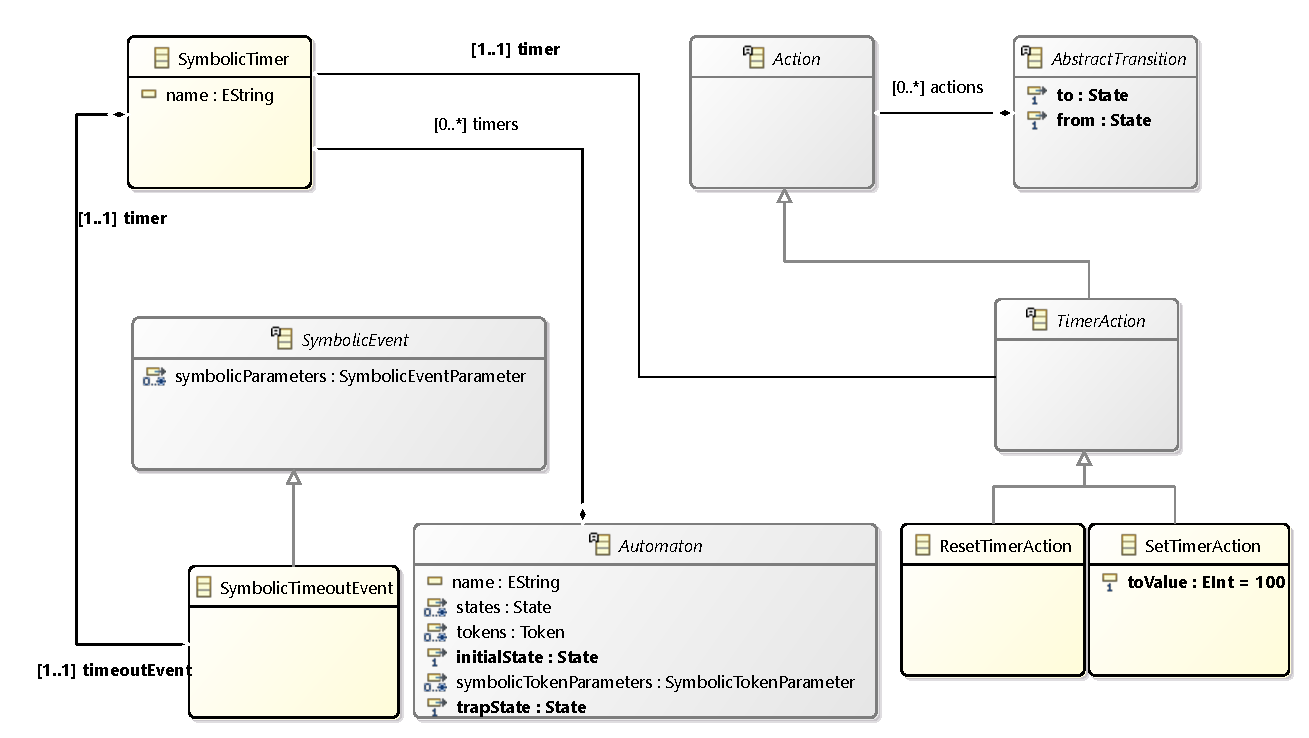
\includegraphics[width=\linewidth]{figures/chapter_5/Timing_diagram}
	\caption{Metamodel of the Timed Event Automaton}
	\label{fig:algo:timed_automaton}
\end{figure}

\subsection{Parameters and Bindings}

The part of the automaton metamodel which is extended with the parametric properties are shown on \cref{fig:algo:parametric_automaton}
The parametrization of the events is represented by the Parameter abstract class. The type of each parameter is implemented with a reference to a SymbolicEvent instance. Parameters can be Fix or Free, an Event only has Fix parameters, but the tokens can have both. Event parameters can be bound to fix values or to a token parameter, this is done by the ConstantBinding and TokenParameterBinding respectively.

\begin{figure}[h]
	\centering
	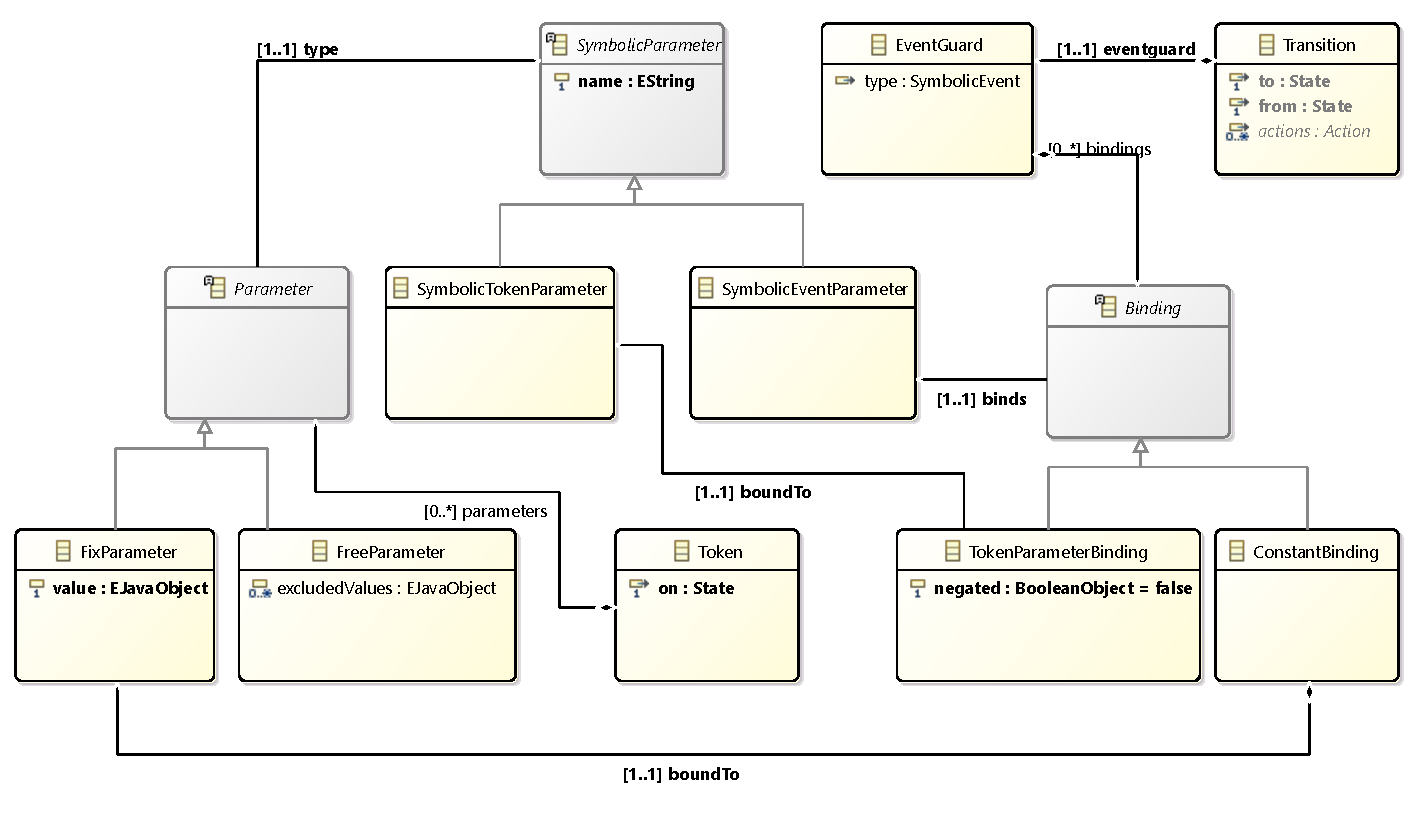
\includegraphics[width=\linewidth]{figures/chapter_5/Parameters_diagram}
	\caption{Metamodel of the Parametric Timed Event Automaton}
	\label{fig:algo:parametric_automaton}
\end{figure}

\subsubsection{Executor}
The algorithm first searches for all the activated transitions.
If it finds an activated transition, it iterates over the tokens which in on that state. The first token with matching (non-confronting)
parameter list will be split to the next state if there are new parameter bindings from the event, or moved if there are no new bindings.
If a token enters an acceptor state it will trigger a function call.

\section{Transformation from VEPL to the intermediate language}


\subsection{VEPL to Regular expressions}
Regular expressions can be built from VEPL patterns, taking the event contexts into consideration
Strict immediate is show on \cref{tab:cep:vepl_regex_strict}, and Chronicle is shown on \cref{tab:cep:vepl_regex_chronicle}.
Each of the patterns must start with a $\Sigma^*$, as in Complex Event Processing every pattern might have arbitrary prefix.


\begin{table}
	\caption{Basic VEPL operators in strict immediate context, expressed with regular expressions}		
	\label{tab:cep:vepl_regex_strict}
	\centering
	\begin{tabularx}{0.5\textwidth}{llX}
		\toprule
		VEPL operator             &	Regular Expression \\
		\midrule
		$p_1$ $\rightarrow$ $p_2$ & $p_1\; p_2$ \\
		$p_1$ OR $p_2$            & $p_1|p_2$ \\
		$p\{\ast\}$               & $p^*$ \\
		$p[t]$                    & $p[t]$ \\ 
		\bottomrule
	\end{tabularx}
\end{table}

\begin{table}
	\caption{Basic VEPL operators in chronicle context, expressed with regular expressions}		
	\label{tab:cep:vepl_regex_chronicle}
	\centering
	\begin{tabularx}{0.5\textwidth}{llX}
		\toprule
		VEPL operator             &	Regular Expression \\
		\midrule
		$p_1$ $\rightarrow$ $p_2$ & $p_1 \; (\Sigma/(p_2))^* \; p_2$ \\
		$p_1$ OR $p_2$            & $p_1|p_2$ \\
		$p\{\ast\}$               & nothing\\
		$p[t]$                    & $p[t]$ \\
		\bottomrule
	\end{tabularx}
\end{table}

\section{Automaton Executor}

	\subsection{Parameter Handling}
	\label{section:algo:paramhandling}

	\subsection{Most Na\"ive approach}
	
	The most na\"ive approach is to keep every potential binding in the memory, for example if there is a pattern $a[i_1]\;b[i_1,\dots,i_n]$ where all parameters are integers and event $a[1]$ happens the state of the memory is shown on \cref{tab:algo:memory}. This indicates that there would be $2^{32^{n-1}}$ objects in the memory, which is not feasible even if $n=3$.\footnote{If each object's size is just 1 bit even then $n=2$ would waste 512MB of memory}
	
	\begin{table}
	\caption{State of the memory on the most na\"ive approach}		
	\label{tab:algo:memory}
	\centering
	\begin{tabular}{ccccc}
		\toprule
		$i_1$ &	$i_2$ & $i_3$ & \dots & $i_n$ \\
		\midrule
		1 	  & 0     & 0     & \dots & 0 \\
		1     & 1     & 0     & \dots & 0 \\
		1     & 0     & 1     & \dots & 0 \\ 
		1     & 1     & 1     & \dots & 0 \\ 
		      &       &\vdots &       &   \\
		1     & 1     & 1     & \dots & 1 \\
		1 	  & 2     & 0     & \dots & 0 \\
		1     & 2     & 1     & \dots & 0 \\
	  	      &       &\vdots &       &   \\
		1     & 2     & 1     & \dots & 1 \\ 
		1     & 2     & 2     & \dots & 0 \\ 
		      &       &\vdots &       &   \\
		1     &$2^{32}$ &$2^{32}$ & \dots & $2^{32}$\\
		\bottomrule
	\end{tabular}
	\end{table}
	
	\subsection{Na\"ive approach}	

	The na\"ive approach is to keep an abstract value for each parameter for each token,
	where the abstract value can be either be
	\begin{itemize}
		\item A concrete value, which shows that for that token the given parameter is bound to that value, i.e.~the given parameter must be exactly that value, or
		\item A list of excluded values which shows that for that token the given parameters values have been reduced by them, i.e.~the given parameter must not be any of the excluded values
	\end{itemize}

	With this approach, every operation seems to be plausible, however a simple counter-example easily shows that the solution is wrong.
	
	Consider the following pattern: $\Sigma^*$ $a[i]$ $\Sigma^*$ $b[i,j]$, i.e.~there must happen an event $a$ with a parameter $i$, and after that there can be any number of events with the functor $b$ with the same first parameter as it was in the first $a$ event. To ease the understanding, the notation will be: The state where the outgoing transition with label $a$ originates will be called $s_0$, the state where the outgoing transition with label $b$ originates will be called $s_1$.
	
	If we would use the na\"ive approach with the input sequence of $a[1]$ $b[1,2]$ $b[1,3]$ the following would happen on reading the inputs one by one:
	\begin{enumerate}
		\item A token would be created on $s_0$ with the binding $i=1$
		\item The token would be split into two, 
	\end{enumerate}

	
	
\chapter{Conclusions and future work}

A formalism was introduced, to provide a language for complex event processing



\section{Future Work}

\paragraph*{Acknowledgments}
\phantomsection
\addcontentsline{toc}{chapter}{Acknowledgments}


First and foremost, I would like to thank my supervisor, \advisori, as without his guidance in the last five years I could not create such a work as this thesis.

I would also like to thank my two other advisors \advisorii, and \advisoriii, without their help in formalization and algorithmization would have been way more cumbersome.

I would like to thank Oszkár Semeráth as without his help the measurements would have been a lot harder.

And last, but not least, I would like to thank Kristóf Marussy, and Bálint Hegyi for helping me with L\textsc{a}T\textsc{e}X and Ti\emph{k}Z related issues, to help me create such a beautiful document.


%\chapter*{Acknowledgments}
%\phantomsection
%\addcontentsline{toc}{chapter}{Acknowledgments}
%
%First and foremost, I would like to thank my supervisor, \advisori, as without his guidance in the last five years I could not create such a work as this thesis.
%I would also like to thank my two other advisors, without \advisorii the process of formalization and algorithmization would have been way more cumbersome, 
%



\appendix
\chapter*{Appendix}

\addcontentsline{toc}{chapter}{Appendix}
\setcounter{chapter}{1} % 1 Because reasons
\numberwithin{equation}{section}
\numberwithin{figure}{section}
\numberwithin{lstlisting}{chapter}

\section{Grammar}

\lstinputlisting[language=Xtext, caption={Xtext grammar for the Parametric Timeout Regular Expression},label={lst:grammar}]{ptregex.xtext}


\printbibliography

\label{page:last}

\end{document}

%%% Local Variables:
%%% mode: latex
%%% TeX-master: nil
%%% End:
